% \part{Tutorials and Guidelines}
\part{教程和指导}

{\Large \emph{by Till Tantau}}

\bigskip
\noindent
% To help you get started with \tikzname, instead of a long installation
% and configuration section, this manual starts with tutorials. They
% explain all the basic and some of the more advanced features of the
% system, without going into all the details. This part also contains
% some guidelines on how you should proceed when creating graphics using
% \tikzname.
为了帮你入门 \tikzname,本手册没有立刻给出长长的安装和配置过程,而是直接从教程开始。这些教程解释了该系统所有基本特性和部分高级特性,并不深入所有细节。这部分还指导你在用 \tikzname 绘图时,如何继续前进。

\vskip3cm

\begin{codeexample}[graphic=white,width=0pt]
\tikz \draw[thick,rounded corners=8pt]
  (0,0) -- (0,2) -- (1,3.25) -- (2,2) -- (2,0) -- (0,2) -- (2,2) -- (0,0) -- (2,0);
\end{codeexample}

% % Copyright 2006 by Till Tantau
%
% This file may be distributed and/or modified
%
% 1. under the LaTeX Project Public License and/or
% 2. under the GNU Free Documentation License.
%
% See the file doc/generic/pgf/licenses/LICENSE for more details.

% \section{Tutorial: A Picture for Karl's Students}
\section{教程:给 Karl 的学生的一张图}

\bohs

% This tutorial is intended for new users of \tikzname. It
% does not give an exhaustive account of all the features of \tikzname,
% just of those that you are likely to use right away. 
该教程是写给 \tikzname\ 的新手的,它并不详细罗列 \tikzname\ 的所有特性,而是只讲那些你可能立马会用到的。

% Karl is a math and chemistry high-school teacher. He used to create
% the graphics in his worksheets and exams using \LaTeX's |{picture}|
% environment. While the results were acceptable, creating the graphics
% often turned out to be a lengthy process. Also, there tended to be
% problems with lines having slightly wrong angles and circles also
% seemed to be hard to get right. Naturally, his students could not care
% less whether the lines had the exact right angles and they find
% Karl's exams too difficult no matter how nicely they were drawn. But
% Karl was never entirely satisfied with the result.
Karl 是一名高中数学和化学老师,他以前用 \LaTeX\ 的 |{picture}| 环境,为习题和考试画图。
尽管结果可以接受,但是绘图通常要花很久,并且还有一些问题,比如线之间有微小的角度错误,圆形好像也很难画对。
当然,他的学生并不关心线之间的角度对不对,因为 Karl 出的试题太难了,画得再好也没用。
但 Karl 对绘图的结果从不满意。

% Karl's son, who was even less satisfied with the results (he did not
% have to take the exams, after all),  told Karl that he might wish
% to try out a new package for creating graphics. A bit confusingly,
% this package seems to have two names: First, Karl had to download and
% install a package called \pgfname. Then it turns out that inside this
% package there is another package called \tikzname, which is supposed to
% stand for ``\tikzname\ ist \emph{kein}  Zeichenprogramm.'' Karl finds this
% all a bit strange and \tikzname\ seems to indicate that the package
% does not do what he needs. However, having used \textsc{gnu}
% software for quite some time and ``\textsc{gnu} not being Unix,''
% there seems to be hope yet. His son assures him that \tikzname's name is
% intended to warn people that \tikzname\ is not a program that you can
% use to draw graphics with your mouse or tablet. Rather, it is more
% like a ``graphics language.''
Karl 的儿子对绘图结果更不满意(毕竟他不要考试),儿子告诉 Karl 他也许愿意试试一个新的宏包来绘图。
令人困惑的是,这个宏包似乎有两个名字:首先 Karl 需要下载和安装一个叫 \pgfname\ 的宏包,接着他发现这个宏包里还有另一个宏包,叫 \tikzname,应该代表“\tikzname\ ist \emph{kein}  Zeichenprogramm”(\tikzname\ 不是一个画图程序)。Karl 觉得有点奇怪,从 \tikzname\ 的名字来看,似乎并不能满足自己的要求。
不过,由于他用过一段时间的 \textsc{gnu} 软件,并且知道“\textsc{gnu}'s Not Unix!”(\textsc{gnu} 不是 Unix)这句典故,因此似乎有点希望。
他儿子告诉他,\tikzname\ 起这个名字,是为了提醒人们,\tikzname\ 不是一个用鼠标和平板画图的程序,相反,它更像是一门“图形语言”。

\eohs

% \subsection{Problem Statement}
\subsection{问题陈述}

\bohs
% Karl wants to put a graphic on the next worksheet for his
% students. He is currently teaching his students about sine and
% cosine. What he would like to have is something that looks like this
% (ideally):
Karl 想在下次学生习题中放一张图,他现在正在教正弦和余弦。他想得到这样的图(理想情况):

\eohs

\noindent
\begin{tikzpicture}
  [scale=3,line cap=round,
   % Styles
   axes/.style=,
   important line/.style={very thick},
   information text/.style={rounded corners,fill=red!10,inner sep=1ex}]

  % Local definitions
  \def\costhirty{0.8660256}

  % Colors
  \colorlet{anglecolor}{green!50!black}
  \colorlet{sincolor}{red}
  \colorlet{tancolor}{orange!80!black}
  \colorlet{coscolor}{blue}

  % The graphic
  \draw[help lines,step=0.5cm] (-1.4,-1.4) grid (1.4,1.4);

  \draw (0,0) circle [radius=1cm];

  \begin{scope}[axes]
    \draw[->] (-1.5,0) -- (1.5,0) node[right] {$x$};
    \draw[->] (0,-1.5) -- (0,1.5) node[above] {$y$};

    \foreach \x/\xtext in {-1, -.5/-\frac{1}{2}, 1}
      \draw[xshift=\x cm] (0pt,1pt) -- (0pt,-1pt) node[below,fill=white] {$\xtext$};

    \foreach \y/\ytext in {-1, -.5/-\frac{1}{2}, .5/\frac{1}{2}, 1}
      \draw[yshift=\y cm] (1pt,0pt) -- (-1pt,0pt) node[left,fill=white] {$\ytext$};
  \end{scope}

  \filldraw[fill=green!20,draw=anglecolor] (0,0) -- (3mm,0pt) arc(0:30:3mm);
  \draw (15:2mm) node[anglecolor] {$\alpha$};

  \draw[important line,sincolor]
    (30:1cm) -- node[left=1pt,fill=white] {$\sin \alpha$} +(0,-.5);

  \draw[important line,coscolor]
    (0,0) -- node[below=2pt,fill=white] {$\cos \alpha$} (\costhirty,0);

  \draw[important line,tancolor] (1,0) --
    node [right=1pt,fill=white]
    {
      $\displaystyle \tan \alpha \color{black}=
      \frac{{\color{sincolor}\sin \alpha}}{\color{coscolor}\cos \alpha}$
    } (intersection of 0,0--30:1cm and 1,0--1,1) coordinate (t);

  \draw (0,0) -- (t);

  \draw[xshift=1.85cm] node [right,text width=6cm,information text]
    {
      % The {\color{anglecolor} angle $\alpha$} is $30^\circ$ in the
      % example ($\pi/6$ in radians). The {\color{sincolor}sine of
      %   $\alpha$}, which is the height of the red line, is
      在本例中,{\color{anglecolor} 角 $\alpha$} 为 $30^\circ$ (等于 $\pi / 6$ 弧度),{\color{sincolor} $\alpha$ 的正弦},也就是红色线段的高度,为
      \[
      {\color{sincolor} \sin \alpha} = 1/2.
      \]
      % By the Theorem of Pythagoras we have ${\color{coscolor}\cos^2 \alpha} +
      % {\color{sincolor}\sin^2\alpha} =1$. Thus the length of the blue
      % line, which is the {\color{coscolor}cosine of $\alpha$}, must be
      根据勾股定理,我们有 ${\color{coscolor}\cos^2 \alpha} + {\color{sincolor}\sin^2\alpha} =1$。因此蓝色线段的长度,也就是~{\color{coscolor} $\alpha$ 的余弦},肯定为
      \[
      {\color{coscolor}\cos\alpha} = \sqrt{1 - 1/4} = \textstyle
      \sqrt{3}/2.
      \]%
      % This shows that {\color{tancolor}$\tan \alpha$}, which is the
      % height of the orange line, is
      由此可以得到~{\color{tancolor} $\tan \alpha$},也就是橙色线段的高度,为
      \[
      {\color{tancolor}\tan\alpha} = \frac{{\color{sincolor} \sin \alpha}}{{\color{coscolor}\cos \alpha}} = 1/\sqrt 3.
      \]%
    };
\end{tikzpicture}


% \subsection{Setting up the Environment}
\subsection{设置环境}

\bohs

% In \tikzname, to draw a picture, at the start of the picture
% you need to tell \TeX\ or \LaTeX\ that you want to start a picture. In
% \LaTeX\ this is done using the environment |{tikzpicture}|, in plain
% \TeX\ you just use |\tikzpicture| to start the picture and
% |\endtikzpicture| to end it.
要在 \tikzname\ 中画一张图片,你需要在图片开头告诉 \TeX\ 或者 \LaTeX\ 你想开始画一张图。
在 \LaTeX\ 中需要用 |{tikzpicture}| 环境,在 plain \TeX\ 中你只要用 |\tikzpicture| 开始图片,再用 |\endtikzpicture| 结束图片。

\eohs

% \subsubsection{Setting up the Environment in \LaTeX}
\subsubsection{设置 \LaTeX\ 中的环境}

% Karl, being a \LaTeX\ user, thus sets up his file as follows:
Karl 是一个 \LaTeX\ 用户,所以他的设置是这样的:

\begin{codeexample}[code only]
\documentclass{article} % say
\usepackage{tikz}
\begin{document}
We are working on
\begin{tikzpicture}
  \draw (-1.5,0) -- (1.5,0);
  \draw (0,-1.5) -- (0,1.5);
\end{tikzpicture}.
\end{document}
\end{codeexample}

\bohs

% When executed, that is, run via |pdflatex| or via |latex| followed by
% |dvips|, the resulting will contain something that looks like this:
当程序执行时,也就是用 |pdflatex|,或者是 |latex| 加上 |dvips|,输出包含这样的内容:

\eohs

\begin{codeexample}[width=7cm]
We are working on
\begin{tikzpicture}
  \draw (-1.5,0) -- (1.5,0);
  \draw (0,-1.5) -- (0,1.5);
\end{tikzpicture}.
\end{codeexample}

\bohs

% Admittedly, not quite the whole picture, yet, but we
% do have the axes established. Well, not quite, but we have the lines
% that make up the axes drawn. Karl suddenly has a sinking feeling
% that the picture is still some way off.
诚然,图还算不上完整,不过我们已经建好坐标轴,还画好组成坐标轴的线了。
Karl 突然有点沮丧,似乎离画完还有不少距离。

% Let's have a more detailed look at the code. First, the package
% |tikz| is loaded. This package is a so-called ``frontend'' to the
% basic \pgfname\ system. The basic layer, which is also described in this
% manual, is somewhat more, well, basic and thus harder to use. The
% frontend makes things easier by providing a simpler syntax.
让我们更仔细地看一下代码。首先导入 |tikz| 库,也就是基础 \pgfname\ 系统所谓的“前端”。
本手册还会提到基本层,更基础也更难用。
这个前端语法更简单,让画图变得更容易了。

% Inside the environment there are two |\draw| commands. They mean:
% ``The path, which is specified following the command up to the
% semicolon, should be drawn.'' The first path is specified
% as |(-1.5,0) -- (0,1.5)|, which means ``a straight line from the point
% at position $(-1.5,0)$ to the point at position $(0,1.5)$.'' Here, the
% positions are specified within a special coordinate system in which,
% initially, one unit is 1cm.
里面有两句 |\draw| 命令,意思是:“从此处到逗号间指定的路径,需要画出来。”
第一条路径指定为 |(-1.5,0) -- (0,1.5)|,意思是:“一条从点 $(-1.5,0)$ 到点 $(-1.5,0)$ 的线”。
在这里,位置是用一个特殊的坐标系统指定的,初始的单位长度是 1cm。

% Karl is quite pleased to note that the environment automatically
% reserves enough space to encompass the picture.
Karl 很高兴地注意到,环境中已经预留了足够的空间来容纳图片。

\eohs

% \subsubsection{Setting up the Environment in Plain \TeX}
\subsubsection{设置 Plain \TeX\ 中的环境}

\bohs

% Karl's wife Gerda, who also happens to be a math teacher, is not a
% \LaTeX\ user, but uses plain \TeX\ since she prefers to do things
% ``the old way.'' She can also use \tikzname. Instead of
% |\usepackage{tikz}| she has to write |\input tikz.tex| and instead of
% |\begin{tikzpicture}| she writes |\tikzpicture| and  instead of
% |\end{tikzpicture}| she writes |\endtikzpicture|.
Karl 的妻子 Gerda,恰好也是一名数学老师,她不是 \LaTeX\ 用户,而是用 plain \TeX\ ,因为她更喜欢“老派的方法”。
她也能用 \tikzname,不过不是 |\usepackage{tikz}|,而是 |\input tikz.tex|,同样,|\begin{tikzpicture}| 和 |\end{tikzpicture}| 也应该换成 |\tikzpicture| 和 |\endtikzpicture|。

% Thus, she would use:
因此她应该用下面的语句:

\eohs

\begin{codeexample}[code only]
%% Plain TeX file
\input tikz.tex
\baselineskip=12pt
\hsize=6.3truein
\vsize=8.7truein
We are working on
\tikzpicture
  \draw (-1.5,0) -- (1.5,0);
  \draw (0,-1.5) -- (0,1.5);
\endtikzpicture.
\bye
\end{codeexample}

\bohs

% Gerda can typeset this file using either |pdftex| or |tex| together
% with |dvips|. \tikzname\ will automatically discern which driver she is
% using. If she wishes to use |dvipdfm| together with |tex|, she
% either needs to modify the file |pgf.cfg| or can write
% |\def\pgfsysdriver{pgfsys-dvipdfm.def}| somewhere \emph{before} she
% inputs |tikz.tex| or |pgf.tex|.
Gerda 既能用 |pdftex| 也能用 |tex| 加 |dvips| 来排版这个文件。
\tikzname\ 会自动识别她用了哪个驱动。
如果她想用 |dvipdfm| 结合 |tex|,她既可以选择修改 |pfg.cfg| 文件,也可以选择在导入 |tikz.tex| 或是 |pgf.tex| 之前加上 |\def\pgfsysdriver{pgfsys-dvipdfm.def}|。

\eohs

% \subsubsection{Setting up the Environment in Con\TeX t}
\subsubsection{设置 Con\TeX t 中的环境}

\bohs

% Karl's uncle Hans uses Con\TeX t. Like Gerda, Hans can also use
% \tikzname. Instead of |\usepackage{tikz}| he says
% |\usemodule[tikz]|. Instead of |\begin{tikzpicture}| he writes
%   |\starttikzpicture| and  instead of |\end{tikzpicture}| he writes
% |\stoptikzpicture|.
Karl 的叔叔 Hans 用 Con\TeX t,Hans 也能像 Gerda 一样使用 \tikzname。
他需要把 |\usepackage{tikz}| 换成 |\usemodule[tikz]|,同样,|\begin{tikzpicture}| 和 |\end{tikzpicture}| 也要换成 |\starttikzpicture| 和 |\stoptikzpicture|。

% His version of the example looks like this:
他的样例代码像这样:

\eohs

\begin{codeexample}[code only]
%% ConTeXt file
\usemodule[tikz]

\starttext
  We are working on
  \starttikzpicture
    \draw (-1.5,0) -- (1.5,0);
    \draw (0,-1.5) -- (0,1.5);
  \stoptikzpicture.
\stoptext
\end{codeexample}

\bohs

% Hans will now typeset this file in the usual way using
% |texexec| or |context|.
Hans 现在就能像平常一样,用 |texexec| 或者 |context| 来排版这个文件了。

\eohs

% \subsection{Straight Path Construction}
\subsection{直线路径创建}

\bohs

% The basic building block of all pictures in \tikzname\ is the path.
% A \emph{path} is a series of straight lines and curves that are
% connected (that is not the whole picture, but let us ignore the
% complications for the moment). You start a path by specifying the
% coordinates of the start position as a point in round brackets, as in
% |(0,0)|. This is followed by a series of ``path extension
% operations.'' The simplest is |--|, which we used already. It must be
% followed by another coordinate and it extends the path in a straight
% line to this new position. For example, if we were to turn the two
% paths of the axes into one path, the following would result:
\tikzname\ 里所有图片的基本单元是路径(path)。
\emph{路径}就是相连的直线和曲线(并不是整个图片都是如此,不过让我们暂时忽略复杂的部分)。
你指定一个起点作为路径开始,圆括号中为点的坐标,比如 |(0,0)|。
紧接着是一系列的“路径扩展操作”,最简单的是 |--|,我们之前用过,它后面必须跟着另一个坐标,它将原来的路径沿直线延伸到新的位置。
比如,如果我们打算把坐标轴的两条路径并成一条,那么会得到下面的结果:

\eohs

\begin{codeexample}[]
\tikz \draw (-1.5,0) -- (1.5,0) -- (0,-1.5) -- (0,1.5);
\end{codeexample}

\bohs

% Karl is a bit confused by the fact that there is no |{tikzpicture}|
% environment, here. Instead, the little command |\tikz| is used. This
% command either takes one argument (starting with an opening brace as in
% |\tikz{\draw (0,0) -- (1.5,0)}|, which yields \tikz{\draw (0,0)
%  --(1.5,0);}) or collects everything up to the next semicolon and
% puts it inside a |{tikzpicture}| environment. As a rule of thumb, all
% \tikzname\ graphic drawing commands must occur as an argument of |\tikz|
% or inside a |{tikzpicture}| environment. Fortunately, the command
% |\draw| will only be defined inside this environment, so there is
% little chance that you will accidentally do something wrong here.
Karl 有点困惑,因为这里没见到 |{tikzpicture}| 环境,而是用了一个小命令 |\tikz|。
这个命令既可以接受单个参数(放在花括号中,比如 |\tikz{\draw (0,0) -- (1.5,0)}| 会生成一条线 \tikz{\draw (0,0) --(1.5,0);}),
也可以将其放到 |{tikzpicture}| 环境中,每句用以分号结尾。
一般来说,所有的 \tikzname\ 绘图命令必须作为 |\tikz| 的参数,或者放在 |{tikzpicture}| 环境里。
幸运的是,|\draw| 命令只定义在这种环境下,因此你很少会有出错的机会。

\eohs

% \subsection{Curved Path Construction}
\subsection{曲线路径创建}

\bohs

% The next thing Karl wants to do is to draw the circle. For this,
% straight lines obviously will not do. Instead, we need some way to
% draw curves. For this, \tikzname\ provides a special syntax. One or two
% ``control points'' are needed. The math behind them is not quite
% trivial, but here is the basic idea: Suppose you are at point $x$ and
% the first control point is $y$. Then the curve will start ``going in
% the direction of~$y$ at~$x$,'' that is, the tangent of the curve at $x$
% will point toward~$y$. Next, suppose the curve should end at $z$ and
% the second support point is $w$. Then the curve will, indeed, end at
% $z$ and the tangent of the curve at point $z$ will go through $w$.
Karl 下一步想做的就是画圆,很明显用直线做不到,所以我们需要一些方法绘制曲线。
为此,\tikzname\ 提供了一个特殊的语法,需要用一到两个“控制点”。
它背后的数学并不简单,但是基本思想是:
假设你位于点 $x$,第一个控制点是 $y$,那么曲线开始时会沿着从 $x$ 到 $y$ 的方向,也就是说,该曲线在点 $x$ 处的切线经过 $y$。
接着,假设曲线的结束点为 $z$,第二个控制点是 $w$,那么该曲线就会在点 $z$ 处结束,并且曲线在点 $z$ 处的切线经过 $w$。

% Here is an example (the control points have been added for clarity):
例子如下(为了更清楚地说明,这里画上了控制点):

\eohs

\begin{codeexample}[]
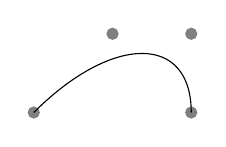
\begin{tikzpicture}
  \filldraw [gray] (0,0) circle [radius=2pt]
                   (1,1) circle [radius=2pt]
                   (2,1) circle [radius=2pt]
                   (2,0) circle [radius=2pt];
  \draw (0,0) .. controls (1,1) and (2,1) .. (2,0);
\end{tikzpicture}
\end{codeexample}

\bohs

% The general syntax for extending a path in a ``curved'' way is
% |.. controls| \meta{first control point} |and| \meta{second control
%   point} |..| \meta{end point}. You can leave out the |and|
% \meta{second control point}, which causes the first one to be used
% twice.
以曲线方式延伸路径的通用语法是 |.. controls| \metazh{第一个控制点} |and| \metazh{第二个控制点} |..| \metazh{结束点}。
你可以略掉 |and| \metazh{第二个控制点},此时第二个控制点和第一个相同。

% So, Karl can now add the first half circle to the picture:
所以,Karl 现在可以把一个半圆加进图片了:

\eohs

\begin{codeexample}[]
\begin{tikzpicture}
  \draw (-1.5,0) -- (1.5,0);
  \draw (0,-1.5) -- (0,1.5);
  \draw (-1,0) .. controls (-1,0.555) and (-0.555,1) .. (0,1)
               .. controls (0.555,1) and (1,0.555) .. (1,0);
\end{tikzpicture}
\end{codeexample}

\bohs

% Karl is happy with the result, but finds specifying circles in this
% way to be extremely awkward. Fortunately, there is a much simpler way.
Karl 看到结果很开心,但是觉得用这种方法指定圆太笨拙了,不过还好有个简单得多的方法。

\eohs

% \subsection{Circle Path Construction}
\subsection{圆形路径创建}

\bohs

% In order to draw a circle, the path construction operation |circle| can
% be used. This operation is followed by a radius in brackets as in
% the following example: (Note that the previous position is used as the
% \emph{center} of the circle.)
路径创建操作 |circle| 可以用来画圆,后面跟着半径,写在方括号里,例子如下:(注意到前面的点作为\emph{圆心}。)

\eohs

\begin{codeexample}[]
\tikz \draw (0,0) circle [radius=10pt];
\end{codeexample}

\bohs

% You can also append an ellipse to the path using the |ellipse|
% operation. Instead of a single radius you can specify two of them:
你还可以用 |ellipse| 画椭圆,它有两个半径:

\eohs

\begin{codeexample}[]
\tikz \draw (0,0) ellipse [x radius=20pt, y radius=10pt];
\end{codeexample}

\bohs

% To draw an ellipse whose axes are not horizontal and vertical, but
% point in an arbitrary direction (a ``turned ellipse'' like \tikz
% \draw[rotate=30] (0,0) ellipse [x radius=6pt, y radius=3pt];) you can use
% transformations, which are explained later. The code for the little
% ellipse is |\tikz \draw[rotate=30] (0,0) ellipse [x radius=6pt, y radius=3pt];|, by
% the way.
要画一个轴线倾斜成任意角度而不是横平竖直的椭圆,比如一个“旋转的椭圆” \tikz \draw[rotate=30] (0,0) ellipse [x radius=6pt, y radius=3pt];,
你可以加上变换,这个后面会解释。
顺带一提,这个小椭圆的代码是:\ltz{\\tikz \\draw[rotate=30] (0,0) ellipse [x radius=6pt, y radius=3pt];}。

% So, returning to Karl's problem, he can write
% |\draw (0,0) circle [radius=1cm];| to draw the circle:
所以,回到 Karl 的问题,他可以用 \ltz{\\draw (0,0) circle [radius=1cm];} 来画圆:

\eohs

\begin{codeexample}[]
\begin{tikzpicture}
  \draw (-1.5,0) -- (1.5,0);
  \draw (0,-1.5) -- (0,1.5);
  \draw (0,0) circle [radius=1cm];
\end{tikzpicture}
\end{codeexample}

\bohs

% At this point, Karl is a bit alarmed that the circle is so small when
% he wants the final picture to be much bigger. He is pleased to learn
% that \tikzname\ has powerful transformation options and scaling
% everything by a factor of three is very easy. But let us leave the
% size as it is for the moment to save some space.
此时 Karl 有点担心,因为这个圆太小了,而他最后想要的图片要大得多。
他很高兴地了解到,\tikzname\ 有强大的变换选项,所以把每样东西都放大三倍非常容易。
不过我们暂时先保留这个尺寸,省点地方。

\eohs

% \subsection{Rectangle Path Construction}
\subsection{矩形路径创建}

\bohs

% The next things we would like to have is the grid in the background.
% There are several ways to produce it. For example, one might draw lots of
% rectangles. Since rectangles are so common, there is a special syntax
% for them: To add a rectangle to the current path, use the |rectangle|
% path construction operation. This operation should be followed by another
% coordinate and will append a rectangle to the path such that the
% previous coordinate and the next coordinates are corners of the
% rectangle. So, let us add two rectangles to the picture:
我们下一步想画背景中的网格,有好几种方法可以实现。
比如你可以画许多矩形。因为矩形很常用,所以有个专门的语法:可以用 |rectangle| 在当前路径中画一个矩形。
这个操作后面需要跟另外一个坐标,这样前后两个坐标就构成了矩形对角的两个点,并将矩形绘制出来。
所以让我们在图片中加两个矩形:

\eohs

\begin{codeexample}[]
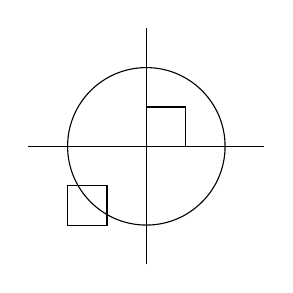
\begin{tikzpicture}
  \draw (-1.5,0) -- (1.5,0);
  \draw (0,-1.5) -- (0,1.5);
  \draw (0,0) circle [radius=1cm];
  \draw (0,0) rectangle (0.5,0.5);
  \draw (-0.5,-0.5) rectangle (-1,-1);
\end{tikzpicture}
\end{codeexample}

\bohs

% While this may be nice in other situations, this is not really leading
% anywhere with Karl's problem: First, we would need an awful lot of
% these rectangles and then there is the border that is not ``closed.''
也许在其他情况下这个方法还不错,但是并没有真的解决 Karl 的问题:首先我们需要很多很多矩形,并且边界处是不“闭合”的。

% So, Karl is about to resort to simply drawing four vertical and four
% horizontal lines using the nice |\draw| command, when he learns that
% there is a |grid| path construction operation.
所以,正当 Karl 准备用 |\draw| 命令画四条横线、四条竖线时,他得知有一个 |grid| (网格)路径创建操作。

\eohs

% \subsection{Grid Path Construction}
\subsection{网格路径创建}

\bohs

% The |grid| path operation adds a grid to the current path. It will add
% lines making up a grid that fills the rectangle whose one corner is
% the current point and whose other corner is the point following the
% |grid| operation. For example, the code
% |\tikz \draw[step=2pt] (0,0) grid (10pt,10pt);| produces \tikz
% \draw[step=2pt] (0,0) grid (10pt,10pt);. Note how the optional
% argument for |\draw| can be used to specify a grid width (there are
% also |xstep| and |ystep| to define the steppings independently). As
% Karl will learn soon, there are \emph{lots} of things that can be
% influenced using such options.
|grid| 路径操作在当前路径加上网格。它会画出组成网格的线,|grid| 前后两个点坐标构成了网格矩形的两个对角。
比如,代码 |\tikz \draw[step=2pt] (0,0) grid (10pt,10pt);| 生成网格 \tikz \draw[step=2pt] (0,0) grid (10pt,10pt);。
注意到 |\draw| 后面的选项,可以指定网格的宽度(还可以用 |xstep| 和 |ystep| 来分别设置网格间隔)。
正如 Karl 很快会学到的,用这些选项可以影响\emph{非常多}的事物。

% For Karl, the following code could be used:
Karl 可以用下面的代码:

\eohs

\begin{codeexample}[]
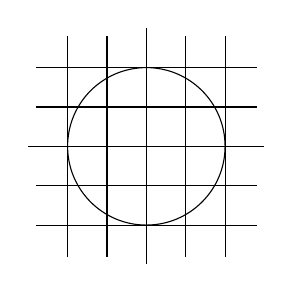
\begin{tikzpicture}
  \draw (-1.5,0) -- (1.5,0);
  \draw (0,-1.5) -- (0,1.5);
  \draw (0,0) circle [radius=1cm];
  \draw[step=.5cm] (-1.4,-1.4) grid (1.4,1.4);
\end{tikzpicture}
\end{codeexample}

\bohs

% Having another look at the desired picture, Karl notices that it would
% be nice for the grid to be more subdued. (His son told him that grids
% tend to be distracting if they are not subdued.) To subdue the grid,
% Karl adds two more options to the |\draw| command that draws the
% grid. First, he uses the color |gray| for the grid lines. Second, he
% reduces the line width to |very thin|. Finally, he swaps the ordering
% of the commands so that the grid is drawn first and everything else on
% top.
Karl 又看了一眼理想中的图片,他注意到,要是网格更柔和一点就好了。%
(他儿子告诉他,如果网格不柔和,会让人分心。)
为了让网格柔和,他又在 |\draw| 后面加了两个选项。
首先他把网格线的颜色设为 |gray|,然后将网格的线宽减到了 |very thin|,最后,他调换了命令的顺序,先画网格,再在上面画其他的。

\eohs

\begin{codeexample}[]
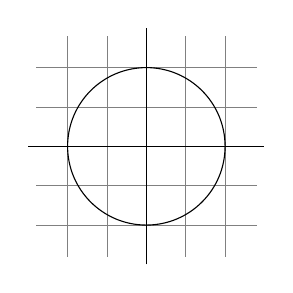
\begin{tikzpicture}
  \draw[step=.5cm,gray,very thin] (-1.4,-1.4) grid (1.4,1.4);
  \draw (-1.5,0) -- (1.5,0);
  \draw (0,-1.5) -- (0,1.5);
  \draw (0,0) circle [radius=1cm];
\end{tikzpicture}
\end{codeexample}


% \subsection{Adding a Touch of Style}
\subsection{加一点样式}

\bohs

% Instead of the options |gray,very thin| Karl could also have
% said |help lines|. \emph{Styles} are predefined sets of options
% that can be used to organize how a graphic is drawn. By saying
% |help lines| you say ``use the style that I (or someone else)
% has set for drawing help lines.'' If Karl decides, at some later
% point, that grids should be drawn, say, using the color |blue!50|
% instead of |gray|, he could provide the following option somewhere:


\eohs

\begin{codeexample}[code only]
help lines/.style={color=blue!50,very thin}
\end{codeexample}

The effect of this ``style setter'' is that in the current
scope or environment the |help lines| option has the same effect as
|color=blue!50,very thin|.

Using styles makes your graphics code more flexible. You can
change the way things look easily in a consistent manner.
Normally, styles are defined at the beginning of a picture. However,
you may sometimes wish to define a style globally, so that all
pictures of your document can use this style. Then you can easily
change the way all graphics look by changing this one style. In this
situation you can use the |\tikzset| command at the beginning of the
document as in
\begin{codeexample}[code only]
\tikzset{help lines/.style=very thin}
\end{codeexample}

To build a hierarchy of styles you can have one style use
another. So in order to define a style |Karl's grid| that is based on
the |grid| style Karl could say
\begin{codeexample}[code only]
\tikzset{Karl's grid/.style={help lines,color=blue!50}}
...
\draw[Karl's grid] (0,0) grid (5,5);
\end{codeexample}

Styles are made even more powerful by parametrization. This means
that, like other options, styles can also be used with a
parameter. For instance, Karl could parameterize his grid so that, by
default, it is blue, but he could also use another color.

\begin{codeexample}[code only]
\begin{tikzpicture}
  [Karl's grid/.style  ={help lines,color=#1!50},
   Karl's grid/.default=blue]

  \draw[Karl's grid]     (0,0) grid (1.5,2);
  \draw[Karl's grid=red] (2,0) grid (3.5,2);
\end{tikzpicture}
\end{codeexample}


\subsection{Drawing Options}

Karl wonders what other options there are that influence how a path is
drawn. He saw already that the |color=|\meta{color} option can be used
to set the line's color. The option |draw=|\meta{color} does nearly
the same, only it sets the color for the lines only and a different
color can be used for filling (Karl will need this when he fills the
arc for the angle).

He saw that the style |very thin| yields very thin lines. Karl is not
really surprised by this and neither is he surprised to learn that |thin|
yields thin lines,  |thick| yields thick lines, |very thick| yields
very thick lines, |ultra thick| yields really, really thick lines and
|ultra thin| yields lines that are so thin that low-resolution printers
and displays will have trouble showing them. He wonders what gives
lines of ``normal'' thickness. It turns out that |thin| is the correct
choice, since it gives the same thickness as \TeX's |\hrule|
command. Nevertheless, Karl would like to know whether there is 
anything ``in the middle'' between |thin| and |thick|. There is:
|semithick|.

Another useful thing one can do with lines is to dash or dot them. For
this, the two styles |dashed| and |dotted| can be used, yielding
\tikz[baseline] \draw[dashed] (0,.5ex) -- ++(2em,0pt); and
\tikz[baseline] \draw[dotted] (0,.5ex) 
-- ++(2em,0pt);. Both options also exist in a loose and a dense
version, called |loosely dashed|, |densely dashed|, |loosely dotted|,
and |densely dotted|. If he really, really  needs to, Karl can also
define much more complex dashing patterns with the |dash pattern|
option, but his son insists that dashing is to be used with utmost
care and mostly distracts. Karl's son claims that complicated dashing
patterns are evil. Karl's students do not care about dashing patterns.



\subsection{Arc Path Construction}

Our next obstacle is to draw the arc for the angle. For this, the
|arc| path construction operation is useful, which draws part of a
circle or ellipse. This |arc| operation is followed by options in
brackets that specify the arc. An example would be \texttt{arc[start
  angle=10, end angle=80, radius=10pt]}, which means exactly what it
says. Karl obviously
needs an arc from $0^\circ$ to $30^\circ$. The radius should be
something relatively small, perhaps around one third of the circle's
radius. When one uses the arc path construction operation, the
specified arc will be added with its starting point at the current
position. So, we first have to ``get there.''

\begin{codeexample}[]
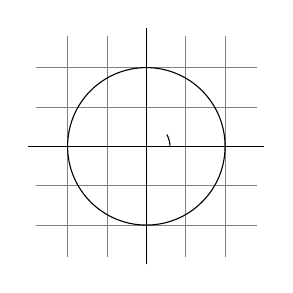
\begin{tikzpicture}
  \draw[step=.5cm,gray,very thin] (-1.4,-1.4) grid (1.4,1.4);
  \draw (-1.5,0) -- (1.5,0);
  \draw (0,-1.5) -- (0,1.5);
  \draw (0,0) circle [radius=1cm];
  \draw (3mm,0mm) arc [start angle=0, end angle=30, radius=3mm];
\end{tikzpicture}
\end{codeexample}

Karl thinks this is really a bit small and he cannot continue unless
he learns how to do scaling. For this, he can add the |[scale=3]|
option. He could add this option to each |\draw| command, but that
would be awkward. Instead, he adds it to the whole environment, which
causes this option to apply to everything within.

\begin{codeexample}[]
\begin{tikzpicture}[scale=3]
  \draw[step=.5cm,gray,very thin] (-1.4,-1.4) grid (1.4,1.4);
  \draw (-1.5,0) -- (1.5,0);
  \draw (0,-1.5) -- (0,1.5);
  \draw (0,0) circle [radius=1cm];
  \draw (3mm,0mm) arc [start angle=0, end angle=30, radius=3mm];
\end{tikzpicture}
\end{codeexample}

As for circles, you can specify ``two'' radii in order to get an
elliptical arc.

\begin{codeexample}[]
  \tikz \draw (0,0) 
    arc [start angle=0, end angle=315, 
         x radius=1.75cm, y radius=1cm];
\end{codeexample}


\subsection{Clipping a Path}

In order to save space in this manual, it would be nice to clip Karl's
graphics a bit so that we can focus on the ``interesting''
parts. Clipping is pretty easy in \tikzname. You can use the |\clip|
command to clip all subsequent drawing. It works like |\draw|, only it
does not draw anything, but uses the given path to clip everything
subsequently.

\begin{codeexample}[]
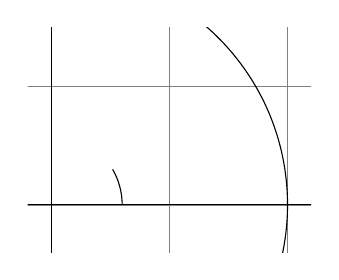
\begin{tikzpicture}[scale=3]
  \clip (-0.1,-0.2) rectangle (1.1,0.75);
  \draw[step=.5cm,gray,very thin] (-1.4,-1.4) grid (1.4,1.4);
  \draw (-1.5,0) -- (1.5,0);
  \draw (0,-1.5) -- (0,1.5);
  \draw (0,0) circle [radius=1cm];
  \draw (3mm,0mm) arc [start angle=0, end angle=30, radius=3mm];
\end{tikzpicture}
\end{codeexample}

You can also do both at the same time: Draw \emph{and} clip a
path. For this, use the |\draw| command and add the |clip|
option. (This is not the whole picture: You can also use the |\clip|
command and add the |draw| option. Well, that is also not the whole
picture: In reality, |\draw| is just a shorthand for |\path[draw]|
and |\clip| is a shorthand for |\path[clip]| and you could also say
|\path[draw,clip]|.) Here is an example:

\begin{codeexample}[]
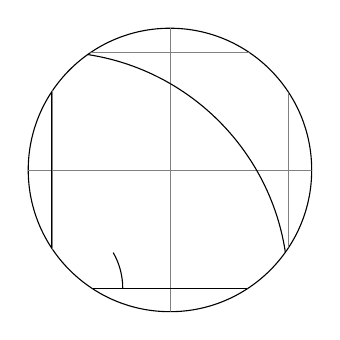
\begin{tikzpicture}[scale=3]
  \clip[draw] (0.5,0.5) circle (.6cm);
  \draw[step=.5cm,gray,very thin] (-1.4,-1.4) grid (1.4,1.4);
  \draw (-1.5,0) -- (1.5,0);
  \draw (0,-1.5) -- (0,1.5);
  \draw (0,0) circle [radius=1cm];
  \draw (3mm,0mm) arc [start angle=0, end angle=30, radius=3mm];
\end{tikzpicture}
\end{codeexample}


\subsection{Parabola and Sine Path Construction}

Although Karl does not need them for his picture, he is pleased to
learn that there are |parabola| and |sin| and |cos| path operations for
adding parabolas and sine and cosine curves to the current path. For the
|parabola| operation, the current point will lie on the parabola as
well as the point given after the parabola operation. Consider
the following example:

\begin{codeexample}[]
\tikz \draw (0,0) rectangle (1,1)  (0,0) parabola (1,1);
\end{codeexample}

It is also possible to place the bend somewhere else:

\begin{codeexample}[]
\tikz \draw[x=1pt,y=1pt] (0,0) parabola bend (4,16) (6,12);
\end{codeexample}

The operations |sin| and |cos| add a sine or cosine curve in the interval
$[0,\pi/2]$ such that the previous current point is at the start of
the curve and the curve ends at the given end point. Here are two
examples:
\begin{codeexample}[]
A sine \tikz \draw[x=1ex,y=1ex] (0,0) sin (1.57,1); curve.
\end{codeexample}

\begin{codeexample}[]
\tikz \draw[x=1.57ex,y=1ex] (0,0) sin (1,1) cos (2,0) sin (3,-1) cos (4,0)
                            (0,1) cos (1,0) sin (2,-1) cos (3,0) sin (4,1);
\end{codeexample}



\subsection{Filling and Drawing}

Returning to the picture, Karl now wants the angle to be ``filled''
with a very light green. For this he uses |\fill| instead of
|\draw|. Here is what Karl does:

\begin{codeexample}[]
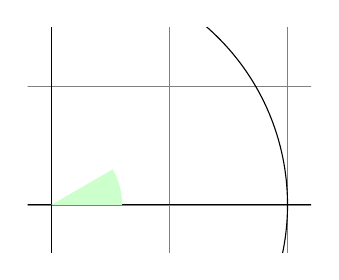
\begin{tikzpicture}[scale=3]
  \clip (-0.1,-0.2) rectangle (1.1,0.75);
  \draw[step=.5cm,gray,very thin] (-1.4,-1.4) grid (1.4,1.4);
  \draw (-1.5,0) -- (1.5,0);
  \draw (0,-1.5) -- (0,1.5);
  \draw (0,0) circle [radius=1cm];
  \fill[green!20!white] (0,0) -- (3mm,0mm)
    arc [start angle=0, end angle=30, radius=3mm] -- (0,0);
\end{tikzpicture}
\end{codeexample}

The color |green!20!white| means 20\% green and 80\% white mixed
together. Such color expression are possible since \tikzname\ uses Uwe
Kern's |xcolor| package, see the documentation of that package for
details on color expressions.

What would have happened, if Karl had not ``closed'' the path using
|--(0,0)| at the end? In this case, the path is closed automatically,
so this could have been omitted. Indeed, it would even have been
better to write the following, instead:
\begin{codeexample}[code only]
  \fill[green!20!white] (0,0) -- (3mm,0mm)
    arc [start angle=0, end angle=30, radius=3mm] -- cycle;
\end{codeexample}
The |--cycle| causes the current path to be closed (actually the
current part of the current path) by smoothly joining the first and
last point. To appreciate the difference, consider the following
example:

\begin{codeexample}[]
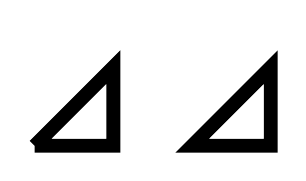
\begin{tikzpicture}[line width=5pt]
  \draw (0,0) -- (1,0) -- (1,1) -- (0,0);
  \draw (2,0) -- (3,0) -- (3,1) -- cycle;
  \useasboundingbox (0,1.5); % make bounding box higher
\end{tikzpicture}
\end{codeexample}

You can also fill and draw a path at the same time using the
|\filldraw| command. This will first draw the path, then fill it. This
may not seem too useful, but you can specify different colors to be
used for filling and for stroking. These are specified as optional
arguments like this:

\begin{codeexample}[]
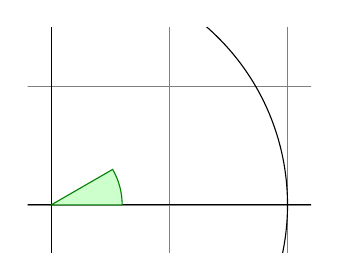
\begin{tikzpicture}[scale=3]
  \clip (-0.1,-0.2) rectangle (1.1,0.75);
  \draw[step=.5cm,gray,very thin] (-1.4,-1.4) grid (1.4,1.4);
  \draw (-1.5,0) -- (1.5,0);
  \draw (0,-1.5) -- (0,1.5);
  \draw (0,0) circle [radius=1cm];
  \filldraw[fill=green!20!white, draw=green!50!black] (0,0) -- (3mm,0mm)
    arc [start angle=0, end angle=30, radius=3mm] -- cycle;
\end{tikzpicture}
\end{codeexample}



\subsection{Shading}

Karl briefly considers the possibility of making the angle ``more
fancy'' by \emph{shading} it. Instead of filling the area with a uniform
color, a smooth transition between different colors is used. For this,
|\shade| and |\shadedraw|, for shading and drawing at the same time,
can be used:

\begin{codeexample}[]
  \tikz \shade (0,0) rectangle (2,1)  (3,0.5) circle (.5cm);
\end{codeexample}
The default shading is a smooth transition from gray to white. To
specify different colors, you can use options:

\begin{codeexample}[]

\begin{tikzpicture}[rounded corners,ultra thick]
  \shade[top color=yellow,bottom color=black] (0,0) rectangle +(2,1);
  \shade[left color=yellow,right color=black] (3,0) rectangle +(2,1);
  \shadedraw[inner color=yellow,outer color=black,draw=yellow] (6,0) rectangle +(2,1);
  \shade[ball color=green] (9,.5) circle (.5cm);
\end{tikzpicture}
\end{codeexample}

For Karl, the following might be appropriate:

\begin{codeexample}[]
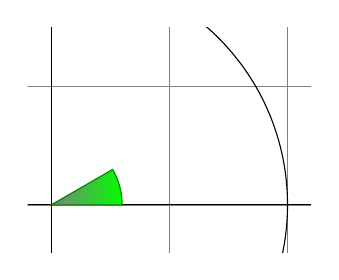
\begin{tikzpicture}[scale=3]
  \clip (-0.1,-0.2) rectangle (1.1,0.75);
  \draw[step=.5cm,gray,very thin] (-1.4,-1.4) grid (1.4,1.4);
  \draw (-1.5,0) -- (1.5,0);
  \draw (0,-1.5) -- (0,1.5);
  \draw (0,0) circle [radius=1cm];
  \shadedraw[left color=gray,right color=green, draw=green!50!black]
    (0,0) -- (3mm,0mm)
    arc [start angle=0, end angle=30, radius=3mm] -- cycle;
\end{tikzpicture}
\end{codeexample}

However, he wisely decides that shadings usually only distract without
adding anything to the picture.


\subsection{Specifying Coordinates}

Karl now wants to add the sine and cosine lines. He knows already that
he can use the |color=| option to set the lines' colors. So, what is
the best way to specify the coordinates?

There are different ways of specifying coordinates. The easiest way is
to say something like |(10pt,2cm)|. This means 10pt in $x$-direction
and 2cm in $y$-directions. Alternatively, you can also leave out the
units as in |(1,2)|, which means ``one times the current $x$-vector
plus twice the current $y$-vector.'' These vectors default to 1cm in
the $x$-direction and 1cm in the $y$-direction, respectively.

In order to specify points in polar coordinates, use the notation
|(30:1cm)|, which means 1cm in direction 30 degree. This is obviously
quite useful to ``get to the point $(\cos 30^\circ,\sin 30^\circ)$ on
the circle.''

You can add a single |+| sign in front of a coordinate or two of
them as in |+(0cm,1cm)| or |++(2cm,0cm)|. Such coordinates are interpreted
differently: The first form means ``1cm upwards from the previous
specified position'' and the second means ``2cm to the right of the
previous specified position, making this the new specified position.''
For example, we can draw the sine line as follows:

\begin{codeexample}[]
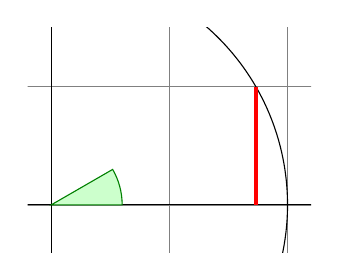
\begin{tikzpicture}[scale=3]
  \clip (-0.1,-0.2) rectangle (1.1,0.75);
  \draw[step=.5cm,gray,very thin] (-1.4,-1.4) grid (1.4,1.4);
  \draw (-1.5,0) -- (1.5,0);
  \draw (0,-1.5) -- (0,1.5);
  \draw (0,0) circle [radius=1cm];
  \filldraw[fill=green!20,draw=green!50!black] (0,0) -- (3mm,0mm)
      arc [start angle=0, end angle=30, radius=3mm] -- cycle;
  \draw[red,very thick] (30:1cm) -- +(0,-0.5);
\end{tikzpicture}
\end{codeexample}

Karl used the fact $\sin 30^\circ = 1/2$. However, he very much
doubts that his students know this, so it would be nice to have a way
of specifying ``the point straight down from |(30:1cm)| that lies on
the $x$-axis.'' This is, indeed, possible using a special syntax: Karl
can write \verb!(30:1cm |- 0,0)!. In general, the meaning of
|(|\meta{p}\verb! |- !\meta{q}|)| is ``the intersection of a vertical
line through $p$ and a horizontal line through $q$.''

Next, let us draw the cosine line. One way would be to say
\verb!(30:1cm |- 0,0) -- (0,0)!. Another way is the following: we
``continue'' from where the sine ends:

\begin{codeexample}[]
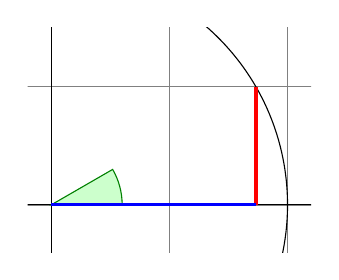
\begin{tikzpicture}[scale=3]
  \clip (-0.1,-0.2) rectangle (1.1,0.75);
  \draw[step=.5cm,gray,very thin] (-1.4,-1.4) grid (1.4,1.4);
  \draw (-1.5,0) -- (1.5,0);
  \draw (0,-1.5) -- (0,1.5);
  \draw (0,0) circle [radius=1cm];
  \filldraw[fill=green!20,draw=green!50!black] (0,0) -- (3mm,0mm)
      arc [start angle=0, end angle=30, radius=3mm] -- cycle;
  \draw[red,very thick]  (30:1cm) -- +(0,-0.5);
  \draw[blue,very thick] (30:1cm) ++(0,-0.5) -- (0,0);
\end{tikzpicture}
\end{codeexample}

Note that there is no |--| between |(30:1cm)| and |++(0,-0.5)|. In
detail, this path is interpreted as follows: ``First, the |(30:1cm)|
tells me to move by pen to $(\cos 30^\circ,1/2)$. Next, there comes
another coordinate specification, so I move my pen there without drawing
anything. This new point is half a unit down from the last position,
thus it is at $(\cos 30^\circ,0)$. Finally, I move the pen to the
origin, but this time drawing something (because of the |--|).''

To appreciate the difference between |+| and |++| consider the
following example:

\begin{codeexample}[]
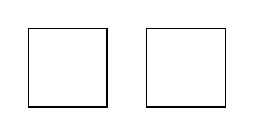
\begin{tikzpicture}
  \def\rectanglepath{-- ++(1cm,0cm)  -- ++(0cm,1cm)  -- ++(-1cm,0cm) -- cycle}
  \draw (0,0) \rectanglepath;
  \draw (1.5,0) \rectanglepath;
\end{tikzpicture}
\end{codeexample}

By comparison, when using a single |+|, the coordinates are different:

\begin{codeexample}[]
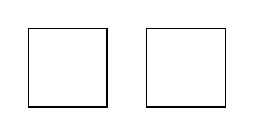
\begin{tikzpicture}
  \def\rectanglepath{-- +(1cm,0cm)  -- +(1cm,1cm)  -- +(0cm,1cm) -- cycle}
  \draw (0,0) \rectanglepath;
  \draw (1.5,0) \rectanglepath;
\end{tikzpicture}
\end{codeexample}


Naturally, all of this could have been written more clearly and more
economically like this (either with a single of a double |+|):
\begin{codeexample}[]
\tikz \draw (0,0) rectangle +(1,1)  (1.5,0) rectangle +(1,1);
\end{codeexample}


\subsection{Intersecting Paths}

Karl is left with the line for $\tan \alpha$, which seems difficult to
specify using transformations and polar coordinates. The first -- and
easiest -- thing he can do is so simply use the coordinate
|(1,{tan(30)})| since \tikzname's math engine knows how to compute
things like |tan(30)|. Note the added braces since, otherwise,
\tikzname's parser would think that the first closing parenthesis ends
the coordinate (in general, you need to add braces around components
of coordinates when these components contain parentheses). 

Karl can, however, also use a more elaborate, but also more
``geometric'' way of computing the length of the orange line: He can
specify intersections of paths as coordinates. The line for $\tan
\alpha$ starts at $(1,0)$ 
and goes upward to a point that is at the intersection of a line going
``up'' and a line going from the origin through |(30:1cm)|. Such
computations are made available by the |intersections| library.

What Karl must do is to create two ``invisible'' paths that intersect
at the position of interest. Creating paths that are not otherwise
seen can be done using the |\path| command without any options like
|draw| or |fill|. Then, Karl can add the |name path| option to the
path for later reference. Once the paths have been constructed, Karl
can use the |name intersections| to assign names to the coordinate for
later reference.

\begin{codeexample}[code only]
\path [name path=upward line] (1,0) -- (1,1);
\path [name path=sloped line] (0,0) -- (30:1.5cm); % a bit longer, so that there is an intersection

\draw [name intersections={of=upward line and sloped line, by=x}]
  [very thick,orange] (1,0) -- (x);
\end{codeexample}


\subsection{Adding Arrow Tips}

Karl now wants to add the little arrow tips at the end of the axes. He has
noticed that in many plots, even in scientific journals, these arrow tips
seem to be missing, presumably because the generating programs cannot
produce them. Karl thinks arrow tips belong at the end of axes. His
son agrees. His students do not care about arrow tips.

It turns out that adding arrow tips is pretty easy: Karl adds the option
|->| to the drawing commands for the axes:

\begin{codeexample}[]
\begin{tikzpicture}[scale=3]
  \clip (-0.1,-0.2) rectangle (1.1,1.51);
  \draw[step=.5cm,gray,very thin] (-1.4,-1.4) grid (1.4,1.4);
  \draw[->] (-1.5,0) -- (1.5,0);
  \draw[->] (0,-1.5) -- (0,1.5);
  \draw (0,0) circle [radius=1cm];
  \filldraw[fill=green!20,draw=green!50!black] (0,0) -- (3mm,0mm)
        arc [start angle=0, end angle=30, radius=3mm] -- cycle;
  \draw[red,very thick]    (30:1cm) -- +(0,-0.5);
  \draw[blue,very thick]   (30:1cm) ++(0,-0.5) -- (0,0);

  \path [name path=upward line] (1,0) -- (1,1);
  \path [name path=sloped line] (0,0) -- (30:1.5cm);
  \draw [name intersections={of=upward line and sloped line, by=x}]
        [very thick,orange] (1,0) -- (x);
\end{tikzpicture}
\end{codeexample}

If Karl had used the option |<-| instead of |->|, arrow tips would
have been put at the beginning of the path. The option |<->| puts
arrow tips at both ends of the path.

There are certain restrictions to the kind of paths to which arrow tips
can be added. As a rule of thumb, you can add arrow tips only to a
single open ``line.'' For example, you cannot add tips to,
say, a rectangle or a circle. However, you can add arrow
tips to curved paths and to paths that have several segments, as in
the following examples:

\begin{codeexample}[]
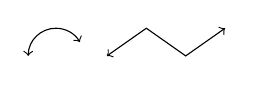
\begin{tikzpicture}
  \draw [<->] (0,0) arc [start angle=180, end angle=30, radius=10pt];
  \draw [<->] (1,0) -- (1.5cm,10pt) -- (2cm,0pt) -- (2.5cm,10pt);
\end{tikzpicture}
\end{codeexample}

Karl has a more detailed look at the arrow that \tikzname\ puts at the
end. It looks like this when he zooms it: \tikz[baseline]
\draw[->,line width=1pt] (0pt,.5ex) -- ++(10pt,0pt);. The shape seems
vaguely familiar and, indeed, this is exactly the end of \TeX's
standard arrow used in something like $f\colon A \to B$.

Karl likes the arrow, especially since it is not ``as thick'' as the
arrows offered by many other packages. However, he expects that,
sometimes, he might need to use some other kinds of arrow.
To do so, Karl can say |>=|\meta{kind of end arrow tip}, where
\meta{kind of end arrow tip} is a special arrow tip specification. For
example, if Karl says |>=Stealth|, then he tells \tikzname\
that he would like  ``stealth-fighter-like'' arrow tips:

\begin{codeexample}[]
\begin{tikzpicture}[>=Stealth]
  \draw [->] (0,0) arc [start angle=180, end angle=30, radius=10pt];
  \draw [<<-,very thick] (1,0) -- (1.5cm,10pt) -- (2cm,0pt) -- (2.5cm,10pt);
\end{tikzpicture}
\end{codeexample}%>>

Karl wonders whether such a military name for the arrow type is really
necessary. He is not really mollified when his son tells him that
Microsoft's PowerPoint uses the same name. He decides to have his
students discuss this at some point.

In addition to |Stealth| there are several other predefined kinds of
arrow tips Karl can choose from, see Section~\ref{section-arrows}. Furthermore,
he can define arrows types himself, if he needs new ones.


\subsection{Scoping}

Karl saw already that there are numerous graphic options that affect how
paths are rendered. Often, he would like to apply certain options to
a whole set of graphic commands. For example, Karl might wish to draw
three paths using a |thick| pen, but would like everything else to
be drawn ``normally.''

If Karl wishes to set a certain graphic option for the whole picture,
he can simply pass this option to the |\tikz| command or to the
|{tikzpicture}| environment (Gerda would pass the options to
|\tikzpicture| and Hans passes them to |\starttikzpicture|). However,
if Karl wants to apply graphic options to a local group, he put these
commands inside a |{scope}| environment (Gerda uses |\scope| and
|\endscope|, Hans uses |\startscope| and |\stopscope|). This
environment takes graphic options as an optional argument and these
options apply to everything inside the scope, but not to anything outside.

Here is an example:

\begin{codeexample}[]
\begin{tikzpicture}[ultra thick]
  \draw (0,0) -- (0,1);
  \begin{scope}[thin]
    \draw (1,0) -- (1,1);
    \draw (2,0) -- (2,1);
  \end{scope}
  \draw (3,0) -- (3,1);
\end{tikzpicture}
\end{codeexample}

Scoping has another interesting effect: Any changes to the clipping
area are local to the scope. Thus, if you say |\clip| somewhere inside
a scope, the effect of the |\clip| command ends at the end of the
scope. This is useful since there is no other way of ``enlarging'' the
clipping area.

Karl has also already seen that giving options to commands like
|\draw| apply only to that command. It turns out that the situation is
slightly more complex. First, options to a command like |\draw| are
not really options to the command, but they are ``path options'' and
can be given anywhere on the path. So, instead of
|\draw[thin] (0,0) -- (1,0);| one can also write
|\draw (0,0) [thin] -- (1,0);| or |\draw (0,0) -- (1,0) [thin];|; all
of these have the same effect. This might seem strange since in the
last case, it would appear that the |thin| should take effect only
``after'' the line from $(0,0)$ to $(1,0)$ has been drawn. However,
most graphic options only apply to the whole path. Indeed, if you say
both |thin| and |thick| on the same path, the last option given will
``win.''

When reading the above, Karl notices that only ``most'' graphic
options apply to the whole path. Indeed, all transformation options do
\emph{not} apply to the whole path, but only to ``everything following
them on the path.'' We will have a more detailed look at this in a
moment. Nevertheless, all options given during a path construction
apply only to this path.



\subsection{Transformations}

When you specify a  coordinate like |(1cm,1cm)|, where is that
coordinate placed on the page? To determine the position, \tikzname,
\TeX, and \textsc{pdf} or PostScript all apply certain transformations
to the given coordinate in order to determine the final position on
the page.

\tikzname\ provides numerous options that allow you to transform
coordinates in \tikzname's private coordinate system. For example, the
|xshift| option allows you to shift all subsequent points by a certain
amount:

\begin{codeexample}[]
\tikz \draw (0,0) -- (0,0.5) [xshift=2pt] (0,0) -- (0,0.5);
\end{codeexample}

It is important to note that you can change transformation ``in the
middle of a path,'' a feature that is not supported by \pdf\
or PostScript. The reason is that \tikzname\ keeps track of its own
transformation matrix.

Here is a more complicated example:
\begin{codeexample}[]

\begin{tikzpicture}[even odd rule,rounded corners=2pt,x=10pt,y=10pt]
  \filldraw[fill=yellow!80!black] (0,0)   rectangle (1,1)
        [xshift=5pt,yshift=5pt]   (0,0)   rectangle (1,1)
                    [rotate=30]   (-1,-1) rectangle (2,2);
\end{tikzpicture}
\end{codeexample}

The most useful transformations are |xshift| and |yshift| for
shifting, |shift| for shifting to a given point as in |shift={(1,0)}|
or |shift={+(0,0)}| (the braces are necessary so that \TeX\ does not
mistake the comma for separating options), |rotate| for rotating by a
certain angle (there is also a |rotate around| for rotating around a
given point), |scale| for scaling by a certain factor, |xscale| and
|yscale| for scaling only in the $x$- or $y$-direction (|xscale=-1| is
a flip), and |xslant| and |yslant| for slanting. If these
transformation and those that I have not mentioned are not
sufficient,  the |cm| option allows you to apply an arbitrary
transformation matrix. Karl's students, by the way, do not know what a
transformation matrix is.



\subsection{Repeating Things: For-Loops}

Karl's next aim is to add little ticks on the axes at positions $-1$,
$-1/2$, $1/2$, and $1$. For this, it would be nice to use some kind of
``loop,'' especially since he wishes to do the same thing at each of
these positions. There are different packages for doing this. \LaTeX\
has its own internal command for this, |pstricks| comes along with the
powerful |\multido| command. All of these can be used together with
\tikzname, so if you are familiar with them, feel free to
use them. \tikzname\ introduces yet another command, called |\foreach|,
which I introduced since I could never remember the syntax of the other
packages. |\foreach| is defined in the package |pgffor| and can be used
independently \tikzname, but \tikzname\ includes it automatically.

In its basic form, the |\foreach| command is easy to use:
\begin{codeexample}[]
\foreach \x in {1,2,3} {$x =\x$, }
\end{codeexample}

The general syntax is |\foreach| \meta{variable}| in {|\meta{list of
    values}|} |\meta{commands}. Inside the \meta{commands}, the
\meta{variable} will be assigned to the different values. If the
\meta{commands} do not start with a brace, everything up to the
next semicolon is used as \meta{commands}.

For Karl and the ticks on the axes, he could use the following code:

\begin{codeexample}[]
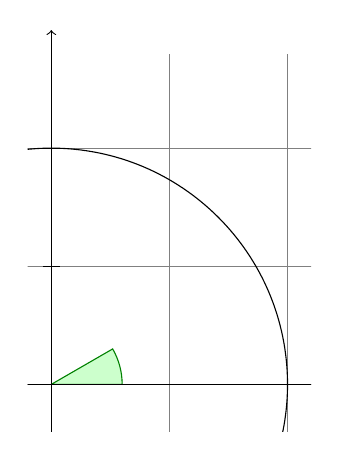
\begin{tikzpicture}[scale=3]
  \clip (-0.1,-0.2) rectangle (1.1,1.51);
  \draw[step=.5cm,gray,very thin] (-1.4,-1.4) grid (1.4,1.4);
  \filldraw[fill=green!20,draw=green!50!black] (0,0) -- (3mm,0mm)
      arc [start angle=0, end angle=30, radius=3mm] -- cycle;
  \draw[->] (-1.5,0) -- (1.5,0);
  \draw[->] (0,-1.5) -- (0,1.5);
  \draw (0,0) circle [radius=1cm];

  \foreach \x in {-1cm,-0.5cm,1cm}
    \draw (\x,-1pt) -- (\x,1pt);
  \foreach \y in {-1cm,-0.5cm,0.5cm,1cm}
    \draw (-1pt,\y) -- (1pt,\y);
\end{tikzpicture}
\end{codeexample}

As a matter of fact, there are many different ways of creating the
ticks. For example, Karl could have put the |\draw ...;| inside curly
braces. He could also have used, say,
\begin{codeexample}[code only]
\foreach \x in {-1,-0.5,1}
  \draw[xshift=\x cm] (0pt,-1pt) -- (0pt,1pt);
\end{codeexample}

Karl is curious what would happen in a more complicated situation
where there are, say, 20 ticks. It seems bothersome to explicitly
mention all these numbers in the set for |\foreach|. Indeed, it is
possible to use |...| inside the |\foreach| statement to iterate over
a large number of values (which must, however, be dimensionless
real numbers) as in the following example:

\begin{codeexample}[]
\tikz \foreach \x in {1,...,10}
        \draw (\x,0) circle (0.4cm);
\end{codeexample}

If you provide \emph{two} numbers before the |...|, the |\foreach|
statement will use their difference for the stepping:

\begin{codeexample}[]
\tikz \foreach \x in {-1,-0.5,...,1}
       \draw (\x cm,-1pt) -- (\x cm,1pt);
\end{codeexample}

We can also nest loops to create interesting effects:

\begin{codeexample}[]
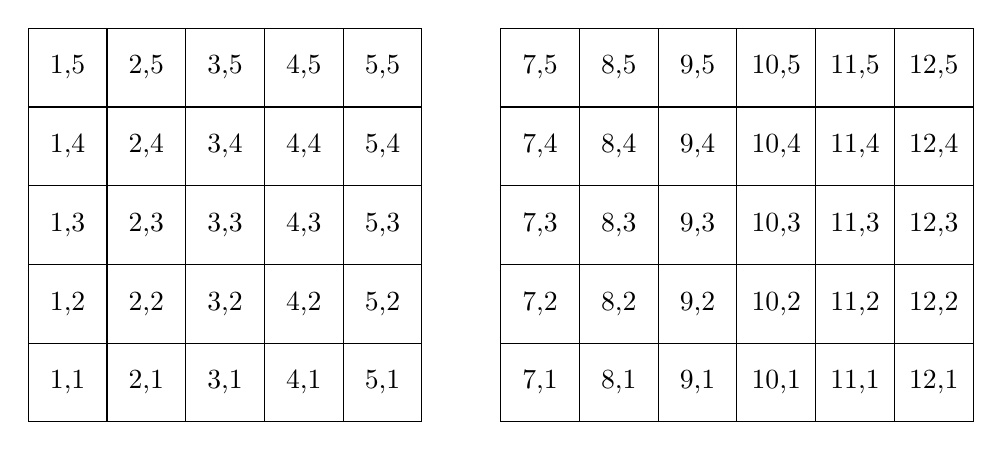
\begin{tikzpicture}
  \foreach \x in {1,2,...,5,7,8,...,12}
    \foreach \y in {1,...,5}
    {
      \draw (\x,\y) +(-.5,-.5) rectangle ++(.5,.5);
      \draw (\x,\y) node{\x,\y};
    }
\end{tikzpicture}
\end{codeexample}

The |\foreach| statement can do even trickier stuff, but the above
gives the idea.




\subsection{Adding Text}

Karl is, by now, quite satisfied with the picture. However, the most
important parts, namely the labels, are still missing!

\tikzname\ offers an easy-to-use and powerful system for adding text and,
more generally, complex shapes to a picture at specific positions. The
basic idea is the following: When \tikzname\ is constructing a path and
encounters the keyword |node| in the middle of a path, it
reads a \emph{node specification}. The keyword |node| is typically
followed by some options and then some text between curly braces. This
text is put inside a normal \TeX\ box (if the node specification
directly follows a coordinate, which is usually the case, \tikzname\ is
able to perform some magic so that it is even possible to use verbatim
text inside the boxes) and then placed at the current position, that
is, at the last specified position (possibly shifted a bit, according
to the given options). However, all nodes are drawn only after the
path has been completely drawn/filled/shaded/clipped/whatever.

\begin{codeexample}[]
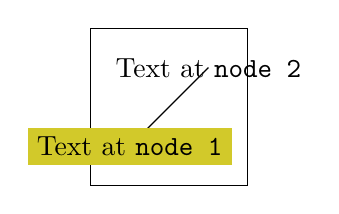
\begin{tikzpicture}
  \draw (0,0) rectangle (2,2);
  \draw (0.5,0.5) node [fill=yellow!80!black]
                       {Text at \verb!node 1!}
     -- (1.5,1.5) node {Text at \verb!node 2!};
\end{tikzpicture}
\end{codeexample}

Obviously, Karl would not only like to place nodes \emph{on} the last
specified position, but also to the left or the
right of these positions. For this, every node object that you
put in your picture is equipped with several \emph{anchors}. For
example, the |north| anchor is in the middle at the upper end of the shape,
the |south| anchor is at the bottom and the |north east| anchor is in
the upper right corner. When you give the option |anchor=north|, the
text will be placed such that this northern anchor will lie on the
current position and the text is, thus, below the current
position. Karl uses this to draw the ticks as follows:

\begin{codeexample}[]
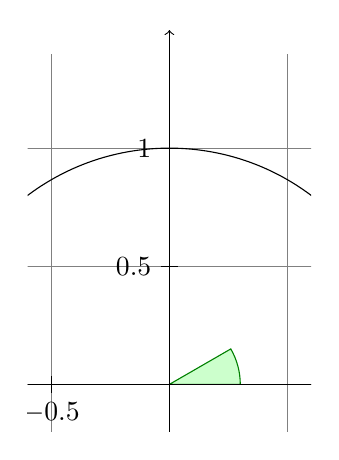
\begin{tikzpicture}[scale=3]
  \clip (-0.6,-0.2) rectangle (0.6,1.51);
  \draw[step=.5cm,help lines] (-1.4,-1.4) grid (1.4,1.4);
  \filldraw[fill=green!20,draw=green!50!black] (0,0) -- (3mm,0mm)
    arc [start angle=0, end angle=30, radius=3mm] -- cycle;
  \draw[->] (-1.5,0) -- (1.5,0);   \draw[->] (0,-1.5) -- (0,1.5);
  \draw (0,0) circle [radius=1cm];

  \foreach \x in {-1,-0.5,1}
    \draw (\x cm,1pt) -- (\x cm,-1pt) node[anchor=north] {$\x$};
  \foreach \y in {-1,-0.5,0.5,1}
    \draw (1pt,\y cm) -- (-1pt,\y cm) node[anchor=east] {$\y$};
\end{tikzpicture}
\end{codeexample}

This is quite nice, already. Using these anchors, Karl can now add
most of the other text elements. However, Karl thinks that, though
``correct,'' it is quite counter-intuitive that in order to place something
\emph{below} a given point, he has to use the \emph{north} anchor. For
this reason, there is an option called |below|, which does the
same as |anchor=north|. Similarly, |above right| does the same as
|anchor=south west|. In addition, |below| takes an optional
dimension argument. If given, the shape will additionally be shifted
downwards by the given amount. So, |below=1pt| can be used to put
a text label below some point and, additionally shift it  1pt
downwards.

Karl is not quite satisfied with the ticks. He would like to have
$1/2$ or $\frac{1}{2}$ shown instead of $0.5$, partly to show off the
nice capabilities of \TeX\ and \tikzname, partly because for positions
like $1/3$ or $\pi$ it is certainly very much preferable to have the
``mathematical'' tick there instead of just the ``numeric'' tick.
His students, on the other hand, prefer $0.5$ over $1/2$
since they are not too fond of fractions in general.

Karl now faces a problem: For the |\foreach| statement, the position
|\x| should still be given as |0.5| since \tikzname\ will not know where
|\frac{1}{2}| is supposed to be. On the other hand, the typeset text
should really be  |\frac{1}{2}|. To solve this problem, |\foreach|
offers a special syntax: Instead of having one variable |\x|, Karl can
specify two (or even more) variables separated by a slash as in
|\x / \xtext|. Then, the elements in the set over which |\foreach|
iterates must also be of the form \meta{first}|/|\meta{second}. In
each iteration, |\x| will be set to \meta{first} and |\xtext| will be
set to \meta{second}. If no \meta{second} is given, the \meta{first}
will be used again. So, here is the new code for the ticks:

\begin{codeexample}[]
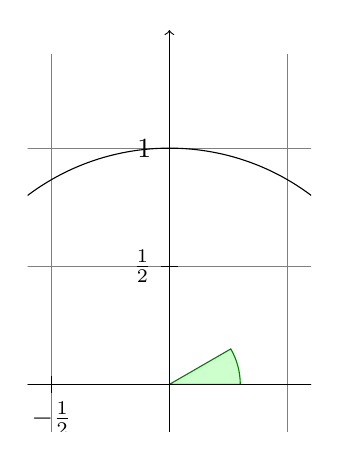
\begin{tikzpicture}[scale=3]
  \clip (-0.6,-0.2) rectangle (0.6,1.51);
  \draw[step=.5cm,help lines] (-1.4,-1.4) grid (1.4,1.4);
  \filldraw[fill=green!20,draw=green!50!black] (0,0) -- (3mm,0mm)
      arc [start angle=0, end angle=30, radius=3mm] -- cycle;
  \draw[->] (-1.5,0) -- (1.5,0); \draw[->] (0,-1.5) -- (0,1.5);
  \draw (0,0) circle [radius=1cm];

  \foreach \x/\xtext in {-1, -0.5/-\frac{1}{2}, 1}
    \draw (\x cm,1pt) -- (\x cm,-1pt) node[anchor=north] {$\xtext$};
  \foreach \y/\ytext in {-1, -0.5/-\frac{1}{2}, 0.5/\frac{1}{2}, 1}
    \draw (1pt,\y cm) -- (-1pt,\y cm) node[anchor=east] {$\ytext$};
\end{tikzpicture}
\end{codeexample}

Karl is quite pleased with the result, but his son points out that
this is still not perfectly satisfactory: The grid and the circle
interfere with the numbers and decrease their legibility. Karl is not
very concerned by this (his students do not even notice), but his son
insists that there is an easy solution: Karl can add the
|[fill=white]| option to fill out the background of the text shape
with a white color.

The next thing Karl wants to do is to add the labels like $\sin
\alpha$. For this, he would like to place a label ``in the middle of
the line.'' To do so, instead of specifying the label
|node {$\sin\alpha$}|  directly after one of the endpoints of the line
(which would place
the label at that endpoint), Karl can give the label directly after
the |--|, before the coordinate. By default, this places the label in
the middle of the line, but the |pos=| options can be used to modify
this. Also, options like |near start| and |near end| can be used to
modify this position:


\begin{codeexample}[]
\begin{tikzpicture}[scale=3]
  \clip (-2,-0.2) rectangle (2,0.8);
  \draw[step=.5cm,gray,very thin] (-1.4,-1.4) grid (1.4,1.4);
  \filldraw[fill=green!20,draw=green!50!black] (0,0) -- (3mm,0mm)
    arc [start angle=0, end angle=30, radius=3mm] -- cycle;
  \draw[->] (-1.5,0) -- (1.5,0) coordinate (x axis);
  \draw[->] (0,-1.5) -- (0,1.5) coordinate (y axis);
  \draw (0,0) circle [radius=1cm];

  \draw[very thick,red]
    (30:1cm) -- node[left=1pt,fill=white] {$\sin \alpha$} (30:1cm |- x axis);
  \draw[very thick,blue]
    (30:1cm |- x axis) -- node[below=2pt,fill=white] {$\cos \alpha$} (0,0);
  \path [name path=upward line] (1,0) -- (1,1);
  \path [name path=sloped line] (0,0) -- (30:1.5cm);
  \draw [name intersections={of=upward line and sloped line, by=t}]
    [very thick,orange] (1,0) -- node [right=1pt,fill=white]
    {$\displaystyle \tan \alpha \color{black}=
      \frac{{\color{red}\sin \alpha}}{\color{blue}\cos \alpha}$} (t);

  \draw (0,0) -- (t);

  \foreach \x/\xtext in {-1, -0.5/-\frac{1}{2}, 1}
    \draw (\x cm,1pt) -- (\x cm,-1pt) node[anchor=north,fill=white] {$\xtext$};
  \foreach \y/\ytext in {-1, -0.5/-\frac{1}{2}, 0.5/\frac{1}{2}, 1}
    \draw (1pt,\y cm) -- (-1pt,\y cm) node[anchor=east,fill=white] {$\ytext$};
\end{tikzpicture}
\end{codeexample}

You can also position labels on curves and, by adding the |sloped|
option, have them rotated such that they match the line's slope. Here
is an example:

\begin{codeexample}[]
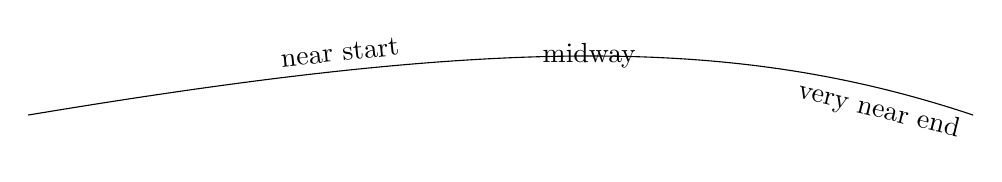
\begin{tikzpicture}
  \draw (0,0) .. controls (6,1) and (9,1) ..
    node[near start,sloped,above] {near start}
    node {midway}
    node[very near end,sloped,below] {very near end} (12,0);
\end{tikzpicture}
\end{codeexample}

It remains to draw the explanatory text at the right of the
picture. The main difficulty here lies in limiting the width of the
text ``label,'' which is quite long, so that line breaking is
used. Fortunately, Karl can use the option |text width=6cm| to get the
desired effect. So, here is the full code:

\begin{codeexample}[code only]
\begin{tikzpicture}
  [scale=3,line cap=round,
  % Styles
  axes/.style=,
  important line/.style={very thick},
  information text/.style={rounded corners,fill=red!10,inner sep=1ex}]

  % Colors
  \colorlet{anglecolor}{green!50!black}
  \colorlet{sincolor}{red}
  \colorlet{tancolor}{orange!80!black}
  \colorlet{coscolor}{blue}

  % The graphic
  \draw[help lines,step=0.5cm] (-1.4,-1.4) grid (1.4,1.4);

  \draw (0,0) circle [radius=1cm];

  \begin{scope}[axes]
    \draw[->] (-1.5,0) -- (1.5,0) node[right] {$x$} coordinate(x axis);
    \draw[->] (0,-1.5) -- (0,1.5) node[above] {$y$} coordinate(y axis);

    \foreach \x/\xtext in {-1, -.5/-\frac{1}{2}, 1}
      \draw[xshift=\x cm] (0pt,1pt) -- (0pt,-1pt) node[below,fill=white] {$\xtext$};

    \foreach \y/\ytext in {-1, -.5/-\frac{1}{2}, .5/\frac{1}{2}, 1}
      \draw[yshift=\y cm] (1pt,0pt) -- (-1pt,0pt) node[left,fill=white] {$\ytext$};
  \end{scope}

  \filldraw[fill=green!20,draw=anglecolor] (0,0) -- (3mm,0pt)
    arc [start angle=0, end angle=30, radius=3mm];
  \draw (15:2mm) node[anglecolor] {$\alpha$};

  \draw[important line,sincolor]
    (30:1cm) -- node[left=1pt,fill=white] {$\sin \alpha$} (30:1cm |- x axis);

  \draw[important line,coscolor]
    (30:1cm |- x axis) -- node[below=2pt,fill=white] {$\cos \alpha$} (0,0);

  \path [name path=upward line] (1,0) -- (1,1);
  \path [name path=sloped line] (0,0) -- (30:1.5cm);
  \draw [name intersections={of=upward line and sloped line, by=t}]
    [very thick,orange] (1,0) -- node [right=1pt,fill=white]
    {$\displaystyle \tan \alpha \color{black}=
      \frac{{\color{red}\sin \alpha}}{\color{blue}\cos \alpha}$} (t);

  \draw (0,0) -- (t);

  \draw[xshift=1.85cm]
    node[right,text width=6cm,information text]
    {
      The {\color{anglecolor} angle $\alpha$} is $30^\circ$ in the
      example ($\pi/6$ in radians). The {\color{sincolor}sine of
        $\alpha$}, which is the height of the red line, is
      \[
      {\color{sincolor} \sin \alpha} = 1/2.
      \]
      By the Theorem of Pythagoras ...
    };
\end{tikzpicture}
\end{codeexample}



\subsection{Pics: The Angle Revisited}

Karl expects that the code of certain parts of the picture he created
might be so useful that he might wish to reuse them in the
future. A natural thing to do is to create \TeX\ macros that store
the code he wishes to reuse. However, \tikzname\ offers another way
that is integrated directly into its parser: pics!

A ``pic'' is ``not quite a full picture,'' hence the short name. The
idea is that a pic is simply some code that you can add to a picture
at different places using the |pic| command whose syntax is almost
identical to the |node| command. The main difference is that instead
of specifying some text in curly braces that should be shown, you
specify the name of a predefined picture that should be shown. 

Defining new pics is easy enough, see Section~\ref{section-pics}, but
right now we just want to use one such predefined pic: the |angle|
pic. As the name suggests, it is a small drawing of an angle
consisting of a little wedge and an arc together with some text (Karl
needs to load the |angle| library and the |quotes| for the following
examples). What makes this pic useful is the fact that the size of the
wedge will be computed automatically.

The |angle| pic draws an angle between the two lines $BA$ and $BC$,
where $A$, $B$, and $C$ are three coordinates. In our case, $B$ is the
origin, $A$ is somewhere on the $x$-axis and $C$ is somewhere on a
line at $30^\circ$. 

\begin{codeexample}[]
\begin{tikzpicture}[scale=3]
  \coordinate (A) at (1,0);
  \coordinate (B) at (0,0);
  \coordinate (C) at (30:1cm);

  \draw (A) -- (B) -- (C)
        pic [draw=green!50!black, fill=green!20, angle radius=9mm,
             "$\alpha$"] {angle = A--B--C};
\end{tikzpicture}  
\end{codeexample}

Let us see, what is happening here. First we have specified three
\emph{coordinates} using the |\coordinate| command. It allows us to
name a specific coordinate in the picture. Then comes something that
starts as a normal |\draw|, but then comes the |pic| command. This
command gets lots of options and, in curly braces, comes the most
important point: We specify that we want to add an |angle| pic and
this angle should be between the points we named |A|, |B|, and |C| (we
could use other names). Note that the text that we want to be shown in
the pic is specified in quotes inside the options of the |pic|, not
inside the curly braces.

To learn more about pics, please see Section~\ref{section-pics}.
% \include{./text-zh/pgfmanual-zh-tutorial/pgfmanual-zh-tutorial-nodes}
% % Copyright 2006 by Till Tantau
%
% This file may be distributed and/or modified
%
% 1. under the LaTeX Project Public License and/or
% 2. under the GNU Free Documentation License.
%
% See the file doc/generic/pgf/licenses/LICENSE for more details.


% \section{Tutorial: Euclid's Amber Version of the \emph{Elements}}
\section{教程:Euclid《几何原本》的琥珀版本}

\bohs

% In this third tutorial we have a look at how \tikzname\ can be used to
% draw geometric constructions.
在这第三篇教程中,我们看看如何用 \tikzname\ 实现几何作图。

% Euclid is currently quite busy writing his new book series, whose
% working title is ``Elements'' (Euclid is not quite sure whether this
% title will convey the message of the series to future generations
% correctly, but he intends to change the title before it goes to the
% publisher). Up to know, he wrote down his text and graphics on
% papyrus, but his publisher suddenly insists that he must submit in
% electronic form. Euclid tries to argue with the publisher that 
% electronics will only be discovered thousands of years later, but the
% publisher informs him that the use of papyrus is no longer cutting edge
% technology and Euclid will just have to keep up with modern tools.
Euclid 最近在忙着写一套新书,书名暂定为“几何原本”(Euclid 不是很确定这个书名是否能把主旨传达给后人,但是他打算在交付给出版商之前修改一下书名)。
到目前为止,他用莎草纸写字画图,但是他的出版商突然要求他必须提交电子版。
Euclid 跟出版商争辩道,电子产品要在几千年后才会发明出来,然而出版商告诉他,莎草纸不再是尖端技术了,他必须得跟上现代工具的步伐。

% Slightly disgruntled, Euclid starts converting his papyrus
% entitled ``Book I, Proposition I'' to an amber version.
Euclid 略带不满,准备把他在莎草纸写的东西转到琥珀上,该部分题为“第 I 卷,命题 1”。

\eohs

% \subsection{Book I, Proposition I}
\subsection{卷 I,命题 1}

\bohs

% The drawing on his papyrus looks like this:\footnote{The text is taken
% from the wonderful interactive version of Euclid's Elements by David
% E. Joyce, to be found on his website at Clark University.}
他在莎草纸上的图是这样的:\footnote{该段文本摘自 David E. Joyce 漂亮的交互式欧几里得几何原本,可以在他 Clark 大学的网站上找到。}
\footnote{{\color{blue} 该段文本原文链接:https://mathcs.clarku.edu/\textasciitilde{}djoyce/java/elements/bookI/propI1.html}}
\footnote{{\color{blue} 该段译文部分参考了:欧几里得\ 著,兰纪正、朱恩宽\ 译. 欧几里得·几何原本. 陕西科学技术出版社, 2003. ISBN 9787536903579.}}

\eohs

% Page 40 of Elements-zh
% 作者:  欧几里得 
% 出版社: 陕西科学技术出版社
% 译者: 兰纪正 / 朱恩宽 
% 出版年: 2003-6
% 页数: 673
% 定价: 38.00元
% ISBN: 9787536903579

\bigskip
\noindent
\begin{tikzpicture}[thick,help lines/.style={thin,draw=black!50}]
  \def\A{\textcolor{input}{$A$}}
  \def\B{\textcolor{input}{$B$}}
  \def\C{\textcolor{output}{$C$}}
  \def\D{$D$}
  \def\E{$E$}
  
  \colorlet{input}{blue!80!black}
  \colorlet{output}{red!70!black}
  \colorlet{triangle}{orange}
  
  \coordinate [label=left:\A]
    (A) at ($ (0,0) + .1*(rand,rand) $);
  \coordinate [label=right:\B]
    (B) at ($ (1.25,0.25) + .1*(rand,rand) $);

  \draw [input] (A) -- (B);
  
  \node [name path=D,help lines,draw,label=left:\D] (D) at (A) [circle through=(B)] {};
  \node [name path=E,help lines,draw,label=right:\E] (E) at (B) [circle through=(A)] {};
  
  \path [name intersections={of=D and E,by={[label=above:\C]C}}];

  \draw [output] (A) -- (C);
  \draw [output] (B) -- (C);

  \foreach \point in {A,B,C}
    \fill [black,opacity=.5] (\point) circle (2pt);

  \begin{pgfonlayer}{background}
    \fill[triangle!80] (A) -- (C) -- (B) -- cycle;
  \end{pgfonlayer}
  
  \node [below right,text width=10cm,align=justify] at (4,3)
  {
    \small
    % \textbf{Proposition I}\par
    \textbf{命题 1}\par
    % \emph{To construct an \textcolor{triangle}{equilateral triangle}
      % on a given \textcolor{input}{finite straight line}.}
    \emph{在一条已知\textcolor{input}{有限直线}上作一个\textcolor{triangle}{等边三角形}.}
    \par
    \vskip1em
    % Let \A\B\ be the given \textcolor{input}{finite straight line}. It
    % is required to construct an \textcolor{triangle}{equilateral
    %   triangle} on the \textcolor{input}{straight line}~\A\B. 
    设 \A\B\ 是已知\textcolor{input}{有限直线}.
    要求在\textcolor{input}{直线} \A\B\ 上作一个\textcolor{triangle}{等边三角形}.

    % Describe the circle \B\C\D\ with center~\A\ and radius \A\B. Again
    % describe the circle \A\C\E\ with center~\B\ and radius \B\A. Join the
    % \textcolor{output}{straight lines} \C\A\ and \C\B\ from the
    % point~\C\ at which the circles cut one another to the points~\A\ and~\B.
    以 \A\ 为中心,\A\B\ 为半径作圆 \B\C\D ;再以 \B\ 为中心,\B\A\ 为半径作圆 \A\C\E ;由两圆交点 \C\ 分别连\textcolor{output}{直线}到 \A 、\B ,得 \C\A 、\C\B .

    % Now, since the point~\A\ is the center of the circle \C\D\B,
    % therefore \A\C\ equals \A\B. Again, since the point \B\ is the
    % center of the circle \C\A\E, therefore \B\C\ equals \B\A. But
    % \A\C\ was proved equal to \A\B, therefore each of the straight
    % lines \A\C\ and \B\C\ equals \A\B. And 
    % things which equal the same thing also equal one another,
    % therefore \A\C\ also equals \B\C. Therefore the three straight
    % lines \A\C, \A\B, and \B\C\ equal one another. 
    % Therefore the \textcolor{triangle}{triangle} \A\B\C\ is
    % equilateral, and it has been  constructed on the given finite
    % \textcolor{input}{straight line}~\A\B.
    因为点 \A\ 为圆 \C\D\B\ 的圆心,所以 \A\C\ 等于 \A\B .
    又因为 \B\ 为圆 \C\A\E\ 的圆心,所以 \B\C\ 等于 \B\A .
    然而已经证明了 \A\C\ 等于 \A\B;所以线段 \A\C\ 、\B\C\ 都等于 \A\B .
    而且等于同量的量彼此相等,因此三条线段 \A\C 、\A\B 和 \B\C\ 彼此相等.
    所以\textcolor{triangle}{三角形} \A\B\C\ 是等边的,并且已经在给定的有限\textcolor{input}{直线} \A\B\ 上作出了该三角形.
  };
\end{tikzpicture}
\bigskip

\bohs

% Let us have a look at how Euclid can turn this into \tikzname\ code.
让我们看看,Euclid 怎么把这张图变成 \tikzname\ 代码。

\eohs

% \subsubsection{Setting up the Environment}
\subsubsection{设置环境}

\bohs

% As in the previous tutorials, Euclid needs to load \tikzname, together
% with some libraries. These libraries are |calc|, |intersections|,
% |through|, and |backgrounds|. Depending on which format he uses,
% Euclid would use one of the following in the preamble:
如之前教程所述,Euclid 需要载入 \tikzname\ 以及一些库,这些库包括 \ltz{calc}、\ltz{intersections}、\ltz{through} 和 \ltz{backgrounds}。
根据格式不同,Euclid 要在序言区加上下列语句之一:

\eohs

\begin{codeexample}[code only]
% 对于 LaTeX:
\usepackage{tikz}
\usetikzlibrary{calc,intersections,through,backgrounds}
\end{codeexample}

\begin{codeexample}[code only]
% 对于 plain TeX:
\input tikz.tex
\usetikzlibrary{calc,intersections,through,backgrounds}
\end{codeexample}

\begin{codeexample}[code only]
% 对于 ConTeXt:
\usemodule[tikz]
\usetikzlibrary[calc,intersections,through,backgrounds]
\end{codeexample}


% \subsubsection{The Line \emph{AB}}
\subsubsection{线 \emph{AB}}

\bohs

% The first part of the picture that Euclid wishes to draw is the line
% $AB$. That is easy enough, something like |\draw (0,0) -- (2,1);|
% might do. However, Euclid does not wish to reference the two points
% $A$ and $B$ as $(0,0)$ and $(2,1)$ subsequently. Rather, he wishes to
% just write |A| and |B|. Indeed, the whole point of his book is that
% the points $A$ and $B$ can be arbitrary and all other points (like
% $C$) are constructed in terms of their positions. It would not do
% if Euclid were to write down the coordinates of $C$ explicitly.
图中 Euclid 想最先画的部分是线 $AB$。很简单,\ltz{\\draw (0,0) -- (2,1);} 就能搞定。
但是,Euclid 不想在 $A$ 和 $B$ 后面加上 $(0,0)$ 和 $(2,1)$,他想只写上 \ltz{A} 和 \ltz{B}。
事实上,他的书的主旨是,点 $A$ 和 $B$ 可以是任意的,其他的点(比如 $C$)可以根据它们的位置构造出来,Euclid 不需要直接写出 $C$ 的坐标。

% So, Euclid starts with defining two coordinates using the
% |\coordinate| command:
所以 Euclid 用 \ltz{\\coordinate} 命令定义两个坐标:

\eohs

\begin{codeexample}[]
\begin{tikzpicture}
  \coordinate (A) at (0,0);
  \coordinate (B) at (1.25,0.25);

  \draw[blue] (A) -- (B);
\end{tikzpicture}
\end{codeexample}

\bohs

% That was easy enough. What is missing at this point are the labels for
% the coordinates. Euclid does not want them \emph{on} the points, but
% next to them. He decides to use the |label| option:
非常简单。
这里少了坐标的标签,Euclid 不想标在点\emph{上面},而是在点旁边。
他决定用 \ltz{label} 选项:

\eohs

\begin{codeexample}[]
\begin{tikzpicture}
  \coordinate [label=left:\textcolor{blue}{$A$}]  (A) at (0,0);
  \coordinate [label=right:\textcolor{blue}{$B$}] (B) at (1.25,0.25);

  \draw[blue] (A) -- (B);
\end{tikzpicture}
\end{codeexample}

\bohs

% At this point, Euclid decides that it would be even nicer if the
% points $A$ and $B$ were in some sense ``random.'' Then, neither Euclid
% nor the reader can make the mistake of taking ``anything for granted''
% concerning these position of these points. Euclid is pleased to learn
% that there is a |rand| function in \tikzname\ that does exactly what
% he needs: It produces a number between $-1$ and $1$. Since \tikzname\
% can do a bit of math, Euclid can change the coordinates of the points
% as follows:
Euclid 这时在想,要是点 $A$ 和 $B$ 可以“随机”一点就更好了。
关于这些点的位置,Euclid 和读者都不能犯下“想当然”的错误。
Euclid 很高兴地了解到,\tikzname\ 里有一个 \ltz{rand} 函数可以满足要求:它能生成一个 $-1$ 到 $1$ 之间的数。
既然 \tikzname\ 能做些数学运算,Euclid 就可以把点坐标写成下面这样:

\eohs

\begin{codeexample}[code only]
\coordinate [...] (A) at (0+0.1*rand,0+0.1*rand);
\coordinate [...] (B) at (1.25+0.1*rand,0.25+0.1*rand);
\end{codeexample}

\bohs

% This works fine. However, Euclid is not quite satisfied since he would
% prefer that the ``main coordinates'' $(0,0)$ and $(1.25,0.25)$ are
% ``kept separate'' from the perturbation
% $0.1(\mathit{rand},\mathit{rand})$. This means, he would like to
% specify that coordinate $A$ as ``The point that is at $(0,0)$ plus one
% tenth of the vector  $(\mathit{rand},\mathit{rand})$.''
这个效果不错,但是 Euclid 并不是很满意,因为他想让“主坐标” $(0,0)$ 和 $(1.25,0.25)$ 同扰动 $0.1(\mathit{rand},\mathit{rand})$ “分离开来”。
也就是说,他希望将坐标 $A$ 指定成这样,“点 $(0,0)$ 加上向量 $(\mathit{rand},\mathit{rand})$ 的十分之一”。

% It turns out that the |calc| library allows him to do exactly this
% kind of computation. When this library is loaded, you can use special
% coordinates that start with |($| and end with |$)| rather than just
% |(| and~|)|. Inside these special coordinates you can give a linear
% combination of coordinates. (Note that the dollar signs are only
% intended to signal that a ``computation'' is going on; no mathematical
% typesetting is done.)
实际上,\ltz{calc} 库来能让他做这类运算。载入该库后,你可以用特殊的坐标,始于 \ltz{($} 止于 \ltz{$)},而不只是 \ltz{(} 和 \ltz{)}。
你可以对这些特殊的坐标进行线性组合。(注意到 \ltz{$} 符号只是表示开始“运算”,而不是输入数学公式。)

% The new code for the coordinates is the following:
关于坐标的新代码如下:

\eohs

\begin{codeexample}[code only]
\coordinate [...] (A) at ($ (0,0) + .1*(rand,rand) $);
\coordinate [...] (B) at ($ (1.25,0.25) + .1*(rand,rand) $);
\end{codeexample}

\bohs

% Note that if a coordinate in such a computation has a factor (like
% |.1|), you must place a |*| directly before the opening parenthesis of
% the coordinate. You can nest such computations.
注意,如果在这类计算中,一个坐标包含小数(比如 \ltz{.1}),那么你必须在坐标的左圆括号之前加上 \ltz{*}。
这些运算可以嵌套。

\eohs

% \subsubsection{The Circle Around \emph{A}}
\subsubsection{围绕点 \emph{A} 的圆}

\bohs

% The first tricky construction is the circle around~$A$. We will see
% later how to do this in a very simple manner, but first let us do it
% the ``hard'' way.
第一个棘手的构造是围绕点 $A$ 的圆。
我们之后会介绍一个非常简单的方法,但是首先让我们用“困难的”方式实现它。

% The idea is the following: We draw a circle around the point $A$ whose
% radius is given by the length of the line $AB$. The difficulty lies in
% computing the length of this line.
思路如下:我们画一个围绕点 $A$ 的圆,其半径由线段 $AB$ 的长度决定。
困难在于计算这条线段的长度。

% Two ideas ``nearly'' solve this problem: First, we can write
% |($ (A) - (B) $)| for the vector that is the difference between $A$
% and~$B$. All we need is the length of this vector. Second, given two
% numbers $x$ and $y$, one can write |veclen(|$x$|,|$y$|)| inside a
% mathematical expression. This gives the value $\sqrt{x^2+y^2}$, which
% is exactly the desired length.
可以通过两个点子解决这个问题:
第一个,我们可以用 \ltz{($ (A) - (B) $)} 表示 $A$ 和 $B$ 相差的向量。
我们需要的是这个向量的长度。
第二个,给定两个数 $x$ 和 $y$,我们可以在数学表达式中写 \ltz{veclen(}{\color{blue} $x$\ltz{,}$y$}\ltz{)},这会返回数值 $\sqrt{x^2+y^2}$,也就是想要的长度。

% The only remaining problem is to access the $x$- and $y$-coordinate of
% the vector~$AB$. For this, we need a new concept: the \emph{let
%   operation}. A let operation can be given anywhere on a path where a
% normal path operation like a line-to or a move-to is expected. The
% effect of a let operation is to evaluate some coordinates and to
% assign the results to special macros. These macros make it easy to
% access the $x$- and $y$-coordinates of the coordinates.
剩下的唯一问题就是如何获得向量 $AB$ 的 $x$ 轴和 $y$ 轴坐标。
为此我们需要引入一个新概念:\ltz{let} \emph{操作}。
\ltz{let} 操作可以在路径中这样一些地方插入,比如直线指向的位置或者移动的目标位置。
\ltz{let} 操作的效果是计算一些坐标并将其结果赋给特定的宏,这些宏方便了对坐标的 $x$ 和 $y$ 值的访问。

% Euclid would write the following:
Euclid 可以这样写:

\eohs

\begin{codeexample}[]
\begin{tikzpicture}
  \coordinate [label=left:$A$]  (A) at (0,0);
  \coordinate [label=right:$B$] (B) at (1.25,0.25);
  \draw (A) -- (B);

  \draw (A) let
              \p1 = ($ (B) - (A) $)
            in
              circle ({veclen(\x1,\y1)});
\end{tikzpicture}
\end{codeexample}

\bohs

% Each assignment in a let operation starts with |\p|, usually followed
% by a \meta{digit}. Then comes an equal sign and a coordinate. The
% coordinate is evaluated and the result is stored internally. From
% then on you can use the following expressions: 
\ltz{let} 操作的每一次赋值都从 \ltz{\\p} 开始,通常跟着一个~{\color{blue}\metazh{数字}},接着是一个等号和一个坐标。
计算好坐标后,结果保存在内部,之后你就可以用下面的表达式:

\eohs

\begin{enumerate}
% \item |\x|\meta{digit} yields the $x$-coordinate of the resulting point.
\item \ltz{\\x}{\color{blue}\metazh{数字}} 得到对应点的 $x$ 坐标。
% \item |\y|\meta{digit} yields the $y$-coordinate of the resulting point.
\item \ltz{\\y}{\color{blue}\metazh{数字}} 得到对应点的 $y$ 坐标。
% \item |\p|\meta{digit} yields the same as |\x|\meta{digit}|,\y|\meta{digit}.
\item \ltz{\\p}{\color{blue}\metazh{数字}} 等同于 \ltz{\\x}{\color{blue}\metazh{数字}}\ltz{,\\y}{\color{blue}\metazh{数字}}。
\end{enumerate}

\bohs

% You can have multiple assignments in a let operation, just separate
% them with commas. In later assignments you can already use the results
% of earlier assignments.
你可以在 \ltz{let} 操作中赋很多值,只要用逗号隔开。
后面的赋值可以使用前面的赋值结果。

% Note that |\p1| is not a coordinate in the usual sense. Rather, it
% just expands to a string like |10pt,20pt|. So, you cannot write, for
% instance, |(\p1.center)| since this would just expand to
% |(10pt,20pt.center)|, which makes no sense.
注意,\ltz{\\p1} 并不是通常意义上的坐标,它只是扩展成 \ltz{10pt,20pt} 这样的字符串。
因此,你不能写 \ltz{(\\p1.center)} 这样的语句,因为这个只会扩展成 \ltz{(10pt,20pt.center)},这条语句没有意义。

% Next, we want to draw both circles at the same time. Each time the
% radius is |veclen(\x1,\y1)|. It seems natural to compute this radius
% only once. For this, we can also use a let operation: Instead of
% writing |\p1 = ...|, we write |\n2 = ...|. Here, ``n'' stands for
% ``number'' (while ``p'' stands for ``point''). The assignment of a
% number should be followed by a number in curly braces.
下一步,我们想同时将两个圆画出来。
两个圆半径都是 \ltz{veclen(\\x1,\\y1)},因此自然只需要计算一次。
这里我们还可以用一个 \ltz{let} 操作:不是写 \ltz{\\p1 = ...},而是写 \ltz{\\n2 = ...}。
这里的 \ltz{n} 表示 “数”(\textbf{n}umber),同理,\ltz{p} 表示“点”(\textbf{p}oint)。
给数赋值需要在外面加上花括号。

\eohs

\begin{codeexample}[]
\begin{tikzpicture}
  \coordinate [label=left:$A$]  (A) at (0,0);
  \coordinate [label=right:$B$] (B) at (1.25,0.25);
  \draw (A) -- (B);

  \draw let \p1 = ($ (B) - (A) $),
            \n2 = {veclen(\x1,\y1)}
        in
          (A) circle (\n2)
          (B) circle (\n2);
\end{tikzpicture}
\end{codeexample}

\bohs

% In the above example, you may wonder, what |\n1| would yield? The
% answer is that it would be undefined -- the |\p|, |\x|, and |\y|
% macros refer to the same logical point, while the |\n| macro has ``its
% own namespace.'' We could even have replaced |\n2| in the example by
% |\n1| and it would still work. Indeed, the digits following these
% macros are just normal \TeX\ parameters. We could also use a longer
% name, but then we have to use curly braces:
看了上例,你可能会想,如果写 \ltz{\\n1} 会得到什么?
答案是会显示它没有定义。
宏 \ltz{\\p}、\ltz{\\x} 和 \ltz{\\y} 引用逻辑上的同一个点,而宏 \ltz{\\n} 则有“自己的命名空间”。
我们甚至可以将例中的 \ltz{\\n2} 替换成 \ltz{\\n1},效果一样。
事实上,跟在这些宏后面的数字只是普通的 \TeX\ 参数。
我们还可以用更长的名字,不过需要加上花括号:

\eohs

\begin{codeexample}[]
\begin{tikzpicture}
  \coordinate [label=left:$A$]  (A) at (0,0);
  \coordinate [label=right:$B$] (B) at (1.25,0.25);
  \draw (A) -- (B);

  \draw let \p1        = ($ (B) - (A) $),
            \n{radius} = {veclen(\x1,\y1)}
        in
          (A) circle (\n{radius})
          (B) circle (\n{radius});
\end{tikzpicture}
\end{codeexample}

\bohs

% At the beginning of this section it was promised that there is an
% easier way to create the desired circle. The trick is to use the
% |through| library. As the name suggests, it contains code for creating
% shapes that go through a given point.
在本节开始我们答应过,有个更简单的方法画出想要的圆。
这个技巧就是用 \ltz{through} 库。
顾名思义,它的作用就是通过一个给定的点创建形状。

% The option that we are looking for is |circle through|. This option is
% given to a \emph{node} and has the following effects: First, it causes
% the node's inner and outer separations to be set to zero. Then it sets
% the shape of the node to |circle|. Finally, it sets the radius of the
% node such that it goes through the parameter given to
% |circle through|. This radius is computed in essentially the same way
% as above.
我们要找的选项是 \ltz{circle through}。
这个选项传给一个\emph{节点},产生如下效果:
首先,它将节点的内外间距置零;然后,将节点的形状设为圆 \ltz{circle};最后,它根据传给 \ltz{circle through} 的参数决定圆的半径,本质上,计算该半径的方法和上面一样。

\eohs

\begin{codeexample}[]
\begin{tikzpicture}
  \coordinate [label=left:$A$]  (A) at (0,0);
  \coordinate [label=right:$B$] (B) at (1.25,0.25);
  \draw (A) -- (B);

  \node [draw,circle through=(B),label=left:$D$] at (A) {};
\end{tikzpicture}
\end{codeexample}


% \subsubsection{The Intersection of the Circles}
\subsubsection{圆的交点}

\bohs

% Euclid can now draw the line and the circles. The final problem is to
% compute the intersection of the two circles. This computation is a bit
% involved if you want to do it ``by hand.'' Fortunately, the
% intersection library allows us to compute the intersection of
% arbitrary paths.
Euclid 现在可以画线和圆了。
最后一个问题就是计算两圆的交点,这就涉及到你是否想“手算”它。
好在 \ltz{intersections} 库可以让我们计算任意路径的交点。

% The idea is simple: First, you ``name'' two paths using the
% |name path| option. Then, at some later point, you can use the option
% |name intersections|, which creates coordinates called
% |intersection-1|, |intersection-2|, and so on at all intersections of
% the paths. Euclid assigns the names |D| and |E| to the paths of the
% two circles (which happen to be the same names as the nodes
% themselves, but nodes and their paths live in different
% ``namespaces''). 
思路很简单:首先用 \ltz{name path} 选项“命名”两条路径;接着,你可以在之后用 \ltz{name intersections} 选项,这会在路径之间的所有交点处创建坐标,名为 \ltz{intersection-1}、\ltz{intersection-2} 等等。
Euclid 将两圆交点命名为 \ltz{D} 和 \ltz{E}(恰好和节点重名,不过节点和路径拥有不同的“命名空间”)。

\eohs

\begin{codeexample}[]
\begin{tikzpicture}
  \coordinate [label=left:$A$]  (A) at (0,0);
  \coordinate [label=right:$B$] (B) at (1.25,0.25);
  \draw (A) -- (B);

  \node (D) [name path=D,draw,circle through=(B),label=left:$D$]  at (A) {};
  \node (E) [name path=E,draw,circle through=(A),label=right:$E$] at (B) {};

  % 给坐标命名,但是什么都不画:
  \path [name intersections={of=D and E}];
  
  \coordinate [label=above:$C$] (C) at (intersection-1);

  \draw [red] (A) -- (C);
  \draw [red] (B) -- (C);
\end{tikzpicture}
\end{codeexample}

\bohs

% It turns out that this can be further shortened: The
% |name intersections| takes an optional argument |by|, which lets you
% specify names for the coordinates and options for them. This creates
% more compact code. Although Euclid does not need it for the current
% picture, it is just a small step to computing the bisection of the line $AB$:
这可以进一步简写:
\ltz{name intersections} 有一个可选参数 \ltz{by},你可以用它指定坐标的名称和选项,这让代码更紧凑。
虽然 Euclid 画现在这张图还用不到,但是画线段 $AB$ 的平分线时,用这个参数只需要一小步。

\eohs

\begin{codeexample}[]
\begin{tikzpicture}
  \coordinate [label=left:$A$]  (A) at (0,0);
  \coordinate [label=right:$B$] (B) at (1.25,0.25);
  \draw [name path=A--B] (A) -- (B);

  \node (D) [name path=D,draw,circle through=(B),label=left:$D$]  at (A) {};
  \node (E) [name path=E,draw,circle through=(A),label=right:$E$] at (B) {};

  \path [name intersections={of=D and E, by={[label=above:$C$]C, [label=below:$C'$]C'}}];

  \draw [name path=C--C',red] (C) -- (C');

  \path [name intersections={of=A--B and C--C',by=F}];
  \node [fill=red,inner sep=1pt,label=-45:$F$] at (F) {};
\end{tikzpicture}
\end{codeexample}

% \subsubsection{The Complete Code}
\subsubsection{完整代码}

\bohs

% Back to Euclid's code. He introduces a few macros to make life
% simpler, like a |\A| macro for typesetting a blue $A$. He also uses the
% |background| layer for drawing the triangle behind everything at the
% end. 
回到 Euclid 的代码,人生苦短,他写了几个宏。比如用 \ltz{\\A} 表示一个蓝色的 $A$,他还用了 \ltz{background} 层,在结尾处画了一个三角形,并置于最底层。

\eohs

\begin{codeexample}[]
\begin{tikzpicture}[thick,help lines/.style={thin,draw=black!50}]
  \def\A{\textcolor{input}{$A$}}     \def\B{\textcolor{input}{$B$}}
  \def\C{\textcolor{output}{$C$}}    \def\D{$D$}
  \def\E{$E$}
  
  \colorlet{input}{blue!80!black}    \colorlet{output}{red!70!black}
  \colorlet{triangle}{orange}
  
  \coordinate [label=left:\A]  (A) at ($ (0,0) + .1*(rand,rand) $);
  \coordinate [label=right:\B] (B) at ($ (1.25,0.25) + .1*(rand,rand) $);

  \draw [input] (A) -- (B);
  
  \node [name path=D,help lines,draw,label=left:\D]   (D) at (A) [circle through=(B)] {};
  \node [name path=E,help lines,draw,label=right:\E]  (E) at (B) [circle through=(A)] {};
  
  \path [name intersections={of=D and E,by={[label=above:\C]C}}];

  \draw [output] (A) -- (C) -- (B);

  \foreach \point in {A,B,C}
    \fill [black,opacity=.5] (\point) circle (2pt);

  \begin{pgfonlayer}{background}
    \fill[triangle!80] (A) -- (C) -- (B) -- cycle;
  \end{pgfonlayer}
  
  \node [below right, text width=10cm,align=justify] at (4,3) {
    \small
    \textbf{命题 1}\par
    \emph{在一条已知\textcolor{input}{有限直线}上作一个\textcolor{triangle}{等边三角形}.}
    \par\vskip1em
    设 \A\B\ 是已知\textcolor{input}{有限直线}. \dots
  };
\end{tikzpicture}
\end{codeexample}

\clearpage
% \subsection{Book I, Proposition II}
\subsection{卷 I,命题 2}

\bohs

% The second proposition in the Elements is the following:
《几何原本》中的第二个命题如下:

\eohs

\bigskip\noindent
\begin{tikzpicture}[thick,help lines/.style={thin,draw=black!50}]
  \def\A{\textcolor{orange}{$A$}}   \def\B{\textcolor{input}{$B$}}
  \def\C{\textcolor{input}{$C$}}    \def\D{$D$}
  \def\E{$E$}                       \def\F{$F$}
  \def\G{$G$}                       \def\H{$H$}
  \def\K{$K$}                       \def\L{\textcolor{output}{$L$}}
  
  \colorlet{input}{blue!80!black}    \colorlet{output}{red!70!black}
  
  \coordinate [label=left:\A]  (A) at ($ (0,0) + .1*(rand,rand) $);
  \coordinate [label=right:\B] (B) at ($ (1,0.2) + .1*(rand,rand) $);
  \coordinate [label=above:\C] (C) at ($ (1,2) + .1*(rand,rand) $);

  \draw [input] (B) -- (C);
  \draw [help lines] (A) -- (B);

  \coordinate [label=above:\D] (D) at ($ (A)!.5!(B) ! {sin(60)*2} ! 90:(B) $);

  \draw [help lines] (D) -- ($ (D)!3.75!(A) $) coordinate [label=-135:\E] (E);
  \draw [help lines] (D) -- ($ (D)!3.75!(B) $) coordinate [label=-45:\F] (F);

  \node (H) at (B) [name path=H,help lines,circle through=(C),draw,label=135:\H] {};
  \path [name path=B--F] (B) -- (F);
  \path [name intersections={of=H and B--F}]
    coordinate [label=right:\G] (G) at (intersection-1);

  \node (K) at (D) [name path=K,help lines,circle through=(G),draw,label=135:\K] {};

  \path [name path=A to E line] (A) -- (E);
  \path [name intersections={of=K and A to E line}]
    coordinate [label=below:\L] (L) at (intersection-1);

  \draw [output] (A) -- (L);

  \foreach \point in {A,B,C,D,G,L}
    \fill [black,opacity=.5] (\point) circle (2pt);
  
  \node [below right, text width=9cm,align=justify] at (4,4) {
    \small
    % \textbf{Proposition II}\par
    \textbf{命题 2} \par
    % \emph{To place a \textcolor{output}{straight line} equal to a
    %   given \textcolor{input}{straight line} with 
    %   one end at a \textcolor{orange}{given point}.} 
    \emph{以一个\textcolor{orange}{已知点}作为端点,作一条\textcolor{output}{线段}与已知\textcolor{input}{线段}相等.}
    \par\vskip1em
    % Let \A\ be the given point, and \B\C\ the given
    % \textcolor{input}{straight line}. 
    % It is required to place a \textcolor{output}{straight line} equal
    % to the given \textcolor{input}{straight line} \B\C\ with one end
    % at the point~\A.  
    设 \A\ 为已知点,\B\C\ 为已知\textcolor{input}{线段}.
    要求以 \A\ 为端点,作一条\textcolor{output}{线段}与已知\textcolor{input}{线段} \B\C\ 相等.

    % Join the straight line \A\B\ from the point \A\ to the point \B, and
    % construct the equilateral triangle \D\A\B\ on it.
    连接点 \A\ 和 \B\ 得线段 \A\B ,并在其上作一等边三角形 \D\A\B .
    
    % Produce the straight lines \A\E\ and \B\F\ in a straight line with
    % \D\A\ and \D\B. Describe the circle \C\G\H\ with center \B\ and
    % radius \B\C, and  again, describe the circle \G\K\L\ with center
    % \D\ and radius \D\G. 	
    延长 \D\A\ 和 \D\B\ 为直线 \A\E\ 和 \B\F 。以 \B\ 为中心,\B\C\ 为半径,作圆 \C\G\H ,再以 \D\ 为中心,\D\G\ 为半径,作圆 \G\K\L .

    % Since the point \B\ is the center of the circle \C\G\H, therefore
    % \B\C\ equals \B\G. Again, since the point \D\ is the center of the
    % circle \G\K\L, therefore \D\L\ equals \D\G. And in these \D\A\
    % equals \D\B, therefore the remainder \A\L\ equals the remainder
    % \B\G. But \B\C\ was also proved  equal to \B\G, therefore each of
    % the straight lines \A\L\ and \B\C\ equals \B\G. And things which
    % equal the same thing also equal one another, therefore \A\L\ also
    % equals \B\C. 
    因为点 \B\ 是圆 \C\G\H\ 的圆心,所以 \B\C\ 等于 \B\G .
    同样,因为点 \D\ 是圆 \G\K\L\ 的圆心,所以 \D\L\ 等于 \D\G .
    又因为 \D\A\ 等于 \D\B ,因此线段之差 \A\L\ 等于线段之差 \B\G .
    然而已经证明了 \B\C\ 等于 \B\G ,所以 \A\L\ 和 \B\C\ 均等于 \B\G .
    而且等于同量的量彼此相等,所以 \A\L\ 也等于 \B\C .

    % Therefore the \textcolor{output}{straight line} \A\L\ equal to the
    % given \textcolor{input}{straight line} \B\C\  has been placed with
    % one end at the \textcolor{orange}{given point}~\A.  
    所以,由已知点 \A\ 作出了\textcolor{output}{线段} \A\L\ ,与已知\textcolor{input}{线段} \B\C\ 相等.
  };
\end{tikzpicture}


% \subsubsection{Using Partway Calculations for the Construction of \emph{D}}
\subsubsection{用分比计算构造点 \emph{D}}

\bohs

% Euclid's construction starts with ``referencing'' Proposition~I for
% the construction of the point~$D$. Now, while we could simply repeat the
% construction, it seems a bit bothersome that one has to draw all these
% circles and do all these complicated constructions.
Euclid 在构造点 $D$ 时,“参考”了命题 1 中的过程。
现在,我们也可以简单重复这些构造过程,但是似乎有点麻烦,因为我们得画出所有这些圆,完成所有复杂的构造。

% For this reason, \tikzname\ supports some simplifications. First,
% there is a simple syntax for computing a point that is ``partway'' on
% a line from $p$ to~$q$: You place these two points in a coordinate
% calculation -- remember, they start with |($| and end with |$)| -- and
% then combine them using |!|\meta{part}|!|. A \meta{part} of |0| refers
% to the \emph{first} coordinate, a \meta{part} of |1| refers to the
% second coordinate, and a value in between refers to a point on the
% line from $p$ to~$q$. Thus, the syntax is similar to the |xcolor|
% syntax for mixing colors.
因此,\tikzname\ 提供了简便方法。
首先,有一个简单的语法,可以计算从 $p$ 到 $q$ 连线上的一点:
将这两个点放到坐标计算环境中——别忘了首尾的 \ltz{($} 和 \ltz{$)}——
然后用 \ltz{!}\metablue{分比}\ltz{!} 将它们组合起来。
\metablue{分比} 为 \ltz{0} 表示 \emph{前面的}坐标,\metablue{分比} 为 \ltz{1} 表示\emph{后面的}坐标,\ltz{0} 到 \ltz{1} 之间的值表示两点连线上的一点。
所以,这个语法类似于 \ltz{xcolor} 中混合颜色的语法。

% Here is the computation of the point in the middle of the line $AB$:
这里展示了如何计算线段 $AB$ 的中点:

\eohs

\begin{codeexample}[]
\begin{tikzpicture}
  \coordinate [label=left:$A$]  (A) at (0,0);
  \coordinate [label=right:$B$] (B) at (1.25,0.25);
  \draw (A) -- (B);
  \node [fill=red,inner sep=1pt,label=below:$X$] (X) at ($ (A)!.5!(B) $) {};
\end{tikzpicture}
\end{codeexample}

\bohs

% The computation of the point $D$ in Euclid's second proposition is a
% bit more complicated. It can be expressed as follows: Consider the
% line from $X$ to $B$. Suppose we 
% rotate this line around $X$ for 90$^\circ$ and then stretch it by a
% factor of $\sin(60^\circ) \cdot 2$. This yields the desired point~$D$. We
% can do the stretching using the partway modifier above, for the
% rotation we need a new modifier: the rotation modifier. The idea is
% that the second coordinate in a partway computation can be prefixed by
% an angle. Then the partway point is computed normally (as if no angle
% were given), but the resulting point is rotated by this angle around
% the first point. 
在 Euclid 的命题 2 中,点 D 的计算更加复杂。
可以表述如下:考虑 $X$ 到 $B$ 的直线,假设我们将该直线以 $X$ 为中心,旋转 90$^\circ$,然后拉伸 $\sin(60^\circ \cdot 2$ 倍,得到点 $D$。
我们可以用上面的分比调节器实现拉伸,然后用另外一个调节器实现旋转。
思路是,在分比计算中,可以在第二个坐标前加上一个角度,接着会正常计算分比得到的点(就像没加角度参数一样),然后再将该点以第一个坐标为心旋转给定的角度。

\eohs

\begin{codeexample}[]
\begin{tikzpicture}
  \coordinate [label=left:$A$]  (A) at (0,0);
  \coordinate [label=right:$B$] (B) at (1.25,0.25);
  \draw (A) -- (B);
  \node [fill=red,inner sep=1pt,label=below:$X$] (X) at ($ (A)!.5!(B) $) {};
  \node [fill=red,inner sep=1pt,label=above:$D$] (D) at
    ($ (X) ! {sin(60)*2} ! 90:(B) $) {};
  \draw (A) -- (D) -- (B);
\end{tikzpicture}
\end{codeexample}

\bohs

% Finally, it is not necessary to explicitly name the point $X$. Rather,
% again like in the |xcolor| package, it is possible to chain partway
% modifiers:
最后,其实不必显式地将点命名为 $X$,而是可以像 \ltz{xcolor} 宏包那样,使用链式语法。

\eohs

\begin{codeexample}[]
\begin{tikzpicture}
  \coordinate [label=left:$A$]  (A) at (0,0);
  \coordinate [label=right:$B$] (B) at (1.25,0.25);
  \draw (A) -- (B);
  \node [fill=red,inner sep=1pt,label=above:$D$] (D) at
    ($ (A) ! .5 ! (B) ! {sin(60)*2} ! 90:(B) $) {};
  \draw (A) -- (D) -- (B);
\end{tikzpicture}
\end{codeexample}


% \subsubsection{Intersecting a Line and a Circle}
\subsubsection{直线和圆相交}

\bohs

% The next step in the construction is to draw a circle around $B$
% through $C$, which is easy enough to do using the |circle through|
% option. Extending the lines $DA$ and $DB$ can be done using partway
% calculations, but this time with a part value outside the range
% $[0,1]$: 
下一步构造是以 $B$ 为圆心,过 $C$ 画一个圆,用 \ltz{circle through} 很容易实现。
延长 $DA$ 和 $DB$ 则可以用分比计算,只不过这次的分比在范围 $[0,1]$ 外:

\eohs

\begin{codeexample}[]
\begin{tikzpicture}
  \coordinate [label=left:$A$]  (A) at (0,0);
  \coordinate [label=right:$B$] (B) at (0.75,0.25);
  \coordinate [label=above:$C$] (C) at (1,1.5);
  \draw (A) -- (B) -- (C);
  \coordinate [label=above:$D$] (D) at
    ($ (A) ! .5 ! (B) ! {sin(60)*2} ! 90:(B) $) {};
  \node (H) [label=135:$H$,draw,circle through=(C)] at (B) {};
  \draw (D) -- ($ (D) ! 3.5 ! (B) $) coordinate [label=below:$F$] (F);
  \draw (D) -- ($ (D) ! 2.5 ! (A) $) coordinate [label=below:$E$] (E);
\end{tikzpicture}
\end{codeexample}

\bohs

% We now face the problem of finding the point $G$, which is the
% intersection of the line $BF$ and the circle $H$. One way is to use
% yet another variant of the partway computation: Normally, a partway
% computation has the form \meta{p}|!|\meta{factor}|!|\meta{q},
% resulting in the point $(1-\meta{factor})\meta{p} +
% \meta{factor}\meta{q}$. Alternatively, instead of \meta{factor} you
% can also use a \meta{dimension} between the points. In this case, you
% get the point that is \meta{dimension} away from \meta{p} on the
% straight line to \meta{q}.
我们现在的问题是如何得到点 $G$,也就是线 $BF$ 和圆 $H$ 的交点。
一个方法是对分比计算进行变形:
正常的分比计算形式是 \metablue{p}\ltz{!}\metablue{分比}\ltz{!}\metablue{q},得到点~{\color{blue} (1 - \metazh{分比}) \meta{p} + \metazh{分比} \meta{q}}。
除了 \metablue{分比}(factor),在两点之间你还可以用 \metablue{长度}(dimension),\footnote{{\color{blue} 关于“分比”一词的原文,作者前面用的是 part,这里用了 factor,为了一致,这里统一译为“分比”。}} \footnote{{\color{blue} dimension 直译应为“维度”、“量纲”或者“尺寸”,但是这里为了更贴合其实际含义,译成了“长度”。}}
这时你得到的点,则在 \metablue{p} 到 \metablue{q} 的直线上,并且到 \metablue{q} 的距离为 \metablue{长度}。


% We know that the point $G$ is on the way from $B$ to $F$. The distance
% is given by the radius of the circle~$H$. Here is the code for
% computing $H$:
我们知道点 $G$ 在 $B$ 到 $F$ 的直线上,$G$ 到 $B$ 的距离等于圆 $H$ 的半径。
计算 $H$ 的代码如下:

\eohs

{\tikzexternaldisable
\begin{codeexample}[pre={
\begin{tikzpicture}
  \coordinate [label=left:$A$]  (A) at (0,0);
  \coordinate [label=right:$B$] (B) at (0.75,0.25);
  \coordinate [label=above:$C$] (C) at (1,1.5);
  \draw (A) -- (B) -- (C);
  \coordinate [label=above:$D$] (D) at
    ($ (A) ! .5 ! (B) ! {sin(60)*2} ! 90:(B) $) {};
  \draw (D) -- ($ (D) ! 3.5 ! (B) $) coordinate [label=below:$F$] (F);
  \draw (D) -- ($ (D) ! 2.5 ! (A) $) coordinate [label=below:$E$] (E);
},post={\end{tikzpicture}}]
  \node (H) [label=135:$H$,draw,circle through=(C)] at (B) {};
  \path let \p1 = ($ (B) - (C) $) in
    coordinate [label=left:$G$] (G) at ($ (B) ! veclen(\x1,\y1) ! (F) $);
  \fill[red,opacity=.5] (G) circle (2pt);
\end{codeexample}

\bohs

% However, there is a simpler way: We can simply name the path of the
% circle and of the line in question and then use |name intersections|
% to compute the intersections.
不过有个更简单的方法:
我们只要给题中圆和线的路径命名,然后用 \ltz{name intersection} 来计算交点。

\eohs

\begin{codeexample}[pre={
\begin{tikzpicture}
  \coordinate [label=left:$A$]  (A) at (0,0);
  \coordinate [label=right:$B$] (B) at (0.75,0.25);
  \coordinate [label=above:$C$] (C) at (1,1.5);
  \draw (A) -- (B) -- (C);
  \coordinate [label=above:$D$] (D) at
    ($ (A) ! .5 ! (B) ! {sin(60)*2} ! 90:(B) $) {};
  \draw (D) -- ($ (D) ! 3.5 ! (B) $) coordinate [label=below:$F$] (F);
  \draw (D) -- ($ (D) ! 2.5 ! (A) $) coordinate [label=below:$E$] (E);
},post={\end{tikzpicture}}]
  \node (H) [name path=H,label=135:$H$,draw,circle through=(C)] at (B) {};
  \path [name path=B--F] (B) -- (F);
  \path [name intersections={of=H and B--F,by={[label=left:$G$]G}}];
  \fill[red,opacity=.5] (G) circle (2pt);
\end{codeexample}
}%

% \subsubsection{The Complete Code}
\subsubsection{完整代码}

\begin{codeexample}[]
\begin{tikzpicture}[thick,help lines/.style={thin,draw=black!50}]
  \def\A{\textcolor{orange}{$A$}}   \def\B{\textcolor{input}{$B$}}
  \def\C{\textcolor{input}{$C$}}    \def\D{$D$}
  \def\E{$E$}                       \def\F{$F$}
  \def\G{$G$}                       \def\H{$H$}
  \def\K{$K$}                       \def\L{\textcolor{output}{$L$}}
  
  \colorlet{input}{blue!80!black}    \colorlet{output}{red!70!black}
  
  \coordinate [label=left:\A]  (A) at ($ (0,0) + .1*(rand,rand) $);
  \coordinate [label=right:\B] (B) at ($ (1,0.2) + .1*(rand,rand) $);
  \coordinate [label=above:\C] (C) at ($ (1,2) + .1*(rand,rand) $);

  \draw [input] (B) -- (C);
  \draw [help lines] (A) -- (B);

  \coordinate [label=above:\D] (D) at ($ (A)!.5!(B) ! {sin(60)*2} ! 90:(B) $);

  \draw [help lines] (D) -- ($ (D)!3.75!(A) $) coordinate [label=-135:\E] (E);
  \draw [help lines] (D) -- ($ (D)!3.75!(B) $) coordinate [label=-45:\F] (F);

  \node (H) at (B) [name path=H,help lines,circle through=(C),draw,label=135:\H] {};
  \path [name path=B--F] (B) -- (F);
  \path [name intersections={of=H and B--F,by={[label=right:\G]G}}];

  \node (K) at (D) [name path=K,help lines,circle through=(G),draw,label=135:\K] {};
  \path [name path=A--E] (A) -- (E);
  \path [name intersections={of=K and A--E,by={[label=below:\L]L}}];

  \draw [output] (A) -- (L);

  \foreach \point in {A,B,C,D,G,L}
    \fill [black,opacity=.5] (\point) circle (2pt);

  % \node ...
\end{tikzpicture}
\end{codeexample}

% \include{./text-zh/pgfmanual-zh-tutorial/pgfmanual-zh-tutorial-chains}
% \include{./text-zh/pgfmanual-zh-tutorial/pgfmanual-zh-tutorial-map}
% % Copyright 2006 by Till Tantau
%
% This file may be distributed and/or modified
%
% 1. under the LaTeX Project Public License and/or
% 2. under the GNU Free Documentation License.
%
% See the file doc/generic/pgf/licenses/LICENSE for more details.


% \section{Guidelines on Graphics}
\section{绘图指导}

\bohs

% The present section is not about \pgfname\ or \tikzname, but about
% general guidelines and principles concerning the creation of
% graphics for scientific presentations, papers, and books.
这一节不是讲 \pgfname\ 和 \tikzname\ 的,而是讲在科学报告、论文和书籍中绘制图形时,通用的指导和原则。

% The guidelines in this section come from different sources. Many of
% them are just what I would like to claim is ``common sense,'' some
% reflect my personal experience (though, hopefully, not my personal
% preferences), some come from books (the bibliography is still missing,
% sorry) on graphic design and typography.
% The most influential source  are the brilliant books
% by Edward Tufte. While I do not agree with everything written in these
% books, many of Tufte's arguments are so convincing that I decided to
% repeat them in the following guidelines.
本节的指导原则源自不同的地方,我想声明的内容,大多都只是“常识”,一些基于我的个人经历(当然,我希望并不只是我个人的偏好),一些来自图形设计和排版的书籍(还没写参考文献,见谅)。

% The first thing you should ask yourself when someone presents a bunch of
% guidelines is: Should I really follow these guidelines? This is an
% important question, because there are good reasons not to follow
% general guidelines.  The person who set up the guidelines may have had other
% objectives than you do. For example, a guideline might say ``use the
% color red for emphasis.'' While this guideline makes perfect sense
% for, say, a presentation using a projector, red ``color'' has the
% \emph{opposite} effect of ``emphasis'' when printed using a
% black-and-white printer. Guidelines were almost always set up to
% address a specific situation. If you are not in this situation,
% following a guideline can do more harm than good.
当有人给你列出一堆指导原则时,你首先得问自己:我真的应该遵循这些指导原则吗?
这是个重要的问题,因为有很多好理由不去遵循这些通用的指导原则。
给出这些指导原则的人,目标可能和你的并不一致。
比如说,某条指导可能写“用红色来强调”,这可能非常适合用投影仪做的报告,但是对于黑白打印的内容来说,红色可能就起了\emph{相反的}效果。
指导原则几乎总是用于处理特定的情况,在错误的情况下遵守它只会弊大于利。

% The second thing you should be aware of is the basic rule of
% typography is: ``Every rule can be broken, as long as you are
% \emph{aware}  that you are breaking a rule.'' This rule also applies
% to graphics. Phrased differently, the basic rule states: ``The only
% mistakes in typography are things done in ignorance.''  When you are
% aware of a rule and when you decide that breaking the rule has a
% desirable effect, break the rule.
关于排版的基本规则,你要知道的第二件事是:“每一条规则都可以打破,只要你确实“意识到”你在打破某条规则。”
这条规则也适用于绘图。
上面那句话换个说法,就是:“排版时唯一的错误,就是对发生的事一无所知。”
如果你想打破一条规则并且清楚后果,那么打破它。

\eohs


% \subsection{Planning the Time Needed for the Creation of Graphics}
\subsection{规划绘图需要的时间}

\bohs

% When you create a paper with numerous graphics, the time needed to
% create these graphics becomes an important factor. How much time
% should you calculate for the creation of graphics?
如果你要写一篇图很多的文章,那么一个重要的因素是,画这些图要花多久。
你怎样计算绘图所需的时间呢?

% As a general rule, assume that a graphic will need as much time to
% create as would a text of the same length. For example, when I
% write a paper, I need about one hour per page for
% the first draft. Later, I need between two and four hours per page
% for revisions. Thus, I expect to need about half an hour for the
% creation of \emph{a first draft} of a half page graphic. Later on, I
% expect another one to two hours before the final graphic is finished.
我们假设,画一张图花费的时间,等于写同样篇幅的文字。
比如我写文章,初稿可能一页一小时,到后面修改时,每页可能需要两到四小时。
那么,要画半页左右的图,\emph{初稿}我预计需要半个小时,后面还需要一到两小时,完成最终的图。

% In many publications, even in good journals, the authors and editors
% have obviously invested a lot of time on the text, but seem to
% have spend about five minutes to create all of the
% graphics. Graphics often seem to have been added as an
% ``afterthought'' or look like a screen shot of whatever the authors's
% statistical software shows them. As will be argued later on, the
% graphics that programs like \textsc{gnuplot} produce by default are of
% poor quality.
在许多出版物甚至是优秀的期刊中,作者和编辑明显在文字上花了很多工夫,但是似乎只花了五分钟就画好了所有图。
通常这些图好像就是“后加上的”,或者只是统计软件的截图。
正如后面会讨论的,像 \textsc{gnuplot} 这种软件默认画出来的图,质量并不高。

% Creating informative graphics that help the reader and that fit
% together with the main text is a difficult, lengthy process.
结合文字绘制信息图,从而帮助读者理解,是一个困难而漫长的过程。

\eohs

\begin{itemize}
\item
  % Treat graphics as first-class citizens of your papers. They deserve
  % as much time and energy as the text does.
  % Indeed, the creation of graphics might deserve \emph{even more} time
  % than the writing of the main text since more attention will be paid
  % to the graphics and they will be looked at first.
  把图形作为你文章的一等公民。图形值得花费同文字相等的时间和精力。
  事实上,相比文字,绘图可能值得投入\emph{更多的}时间,因为人们第一眼看到的就是图形,也更关注图形。
\item
  % Plan as much time for the creation and revision of a graphic as you
  % would plan for text of the same size.
  给图形的绘制和修改规划尽可能多的时间,就像对待同等篇幅的文字一样。
\item
  % Difficult graphics with a high information density may require even
  % more time.
  信息量大的困难的图形,可能需要更多的时间。
\item
  % Very simple graphics will require less time, but most likely you do
  % not want to have ``very simple graphics'' in your paper, anyway;
  % just as you would not like to have a ``very simple text'' of the
  % same size.
  简单的图形需要更少的时间,但是无论如何,很可能你并不想在文章里放“非常简单的图”,就像你不想在文章中写同等篇幅“非常简单的文字”一样。
\end{itemize}


% \subsection{Workflow for Creating a Graphic}
\subsection{绘图的工作流程}

\bohs

% When you write a (scientific) paper, you will most likely follow the
% following pattern: You have some results/ideas that you would
% like to report about. The creation of the paper will typically start
% with compiling a rough outline. Then, the different sections are
% filled with text to create a first draft. This draft is then revised
% repeatedly until, often after substantial revision, a final paper
% results. In a good journal paper there is typically not be a single
% sentence that has survived unmodified from the first draft.
你写一篇(科学)文章,通常会遵循下面的模式:
你有一些结果或者想法要阐述。写文章时一般会先列一个粗糙的大纲,然后分别写各个章节,得到初稿。在成稿写好前,一般要不停地大量地修改。
一篇好的期刊文章,初稿里几乎没有一句到最后还没改过的。

% Creating a graphics follows the same pattern:
绘图也遵循相同的模式:

\eohs

\begin{itemize}
\item
  % Decide on what the graphic should communicate. Make this a conscious
  % decision, that is, determine ``What is the graphic supposed to tell
  % the reader?''
  决定图形想要表达什么。一定要有意识地思考,“图形应该告诉读者什么?”
\item
  % Create an ``outline,'' that is, the rough overall ``shape'' of the
  % graphic, containing the most crucial elements. Often, it is
  % useful to do this using pencil and paper.
  列一个“大纲”,也就是图形整体的大致“轮廓”,包含最重要的元素。
  在这一步,笔纸一般很有帮助。
\item
  % Fill out the finer details of the graphic to create a first
  % draft.
  补充和完善图形的细节,得到初稿。
\item
  % Revise the graphic repeatedly along with the rest of the paper.
  根据文章内容,不断修改图形。
\end{itemize}


% \subsection{Linking Graphics With the Main Text}
\subsection{Linking Graphics With the Main Text}

\bohs

Graphics can be placed at different places in a text. Either, they can
be inlined, meaning they are somewhere ``in the middle of the text''
or they can be placed in stand-alone ``figures.'' Since printers (the
people) like to have their pages ``filled,'' (both for aesthetic and
economic reasons) stand-alone figures may traditionally be placed on
pages in the document far away from the main text that refers to
them. \LaTeX\ and \TeX\ tend to encourage this ``drifting away'' of
graphics for technical reasons.

When a graphic is inlined, it will more or less automatically be
linked with the main text in the sense that the labels of the graphic
will be implicitly explained by the surrounding text. Also, the main
text will typically make it clear what the graphic is about and what
is shown.

Quite differently, a stand-alone figure will often be viewed at a time
when the main text that this graphic belongs to either has not yet
been read or has been read some time ago. For this reason, you should
follow the following guidelines when creating stand-alone figures:

\eohs

\begin{itemize}
\item
  Stand-alone figures should have a caption than should make them
  ``understandable by themselves.''

  For example, suppose a graphic shows an example of the different
  stages of a quicksort algorithm. Then the figure's caption should,
  at the very least, inform the reader that ``The figure shows the
  different stages of the quicksort algorithm introduced on page
  xyz.'' and not just ``Quicksort algorithm.''
\item
  A good caption adds as much context information as possible. For
  example, you could say: ``The figure shows the different stages of
  the quicksort algorithm introduced on page xyz. In the first line,
  the pivot element 5 is chosen. This causes\dots'' While this
  information can also be given in the main text, putting it in the
  caption will ensure that the context is kept. Do not feel afraid of
  a 5-line caption. (Your editor may hate you for this. Consider
  hating them back.)
\item
  Reference the graphic in your main text as in ``For an example of
  quicksort `in action,' see Figure~2.1 on page xyz.''
\item
  Most books on style and typography recommend that you do not use
  abbreviations as in ``Fig.~2.1'' but write ``Figure 2.1.''

  The main argument against abbreviations is that ``a period is too
  valuable to waste it on an abbreviation.'' The idea is that a period
  will make the reader assume that the sentence ends after ``Fig'' and
  it takes a ``conscious backtracking'' to realize that the sentence
  did not end after all.

  The argument in favor of abbreviations is that they save space.

  Personally, I am not really convinced by either argument. On the one
  hand, I have not yet seen any hard evidence that abbreviations slow
  readers down. On the other hand,  abbreviating all ``Figure'' by
  ``Fig.''\ is most unlikely to save even a single line in  most
  documents. I avoid abbreviations.
\end{itemize}



\subsection{Consistency Between Graphics and Text}

Perhaps the most common ``mistake'' people do when creating graphics
(remember that a ``mistake'' in design is always just ``ignorance'')
is to have a mismatch between the way their graphics look and the way
their text looks.

It is quite common that authors use several different programs for
creating the graphics of a paper. An author might produce some plots
using \textsc{gnuplot}, a diagram using \textsc{xfig}, and include an
|.eps| graphic a coauthor contributed using some unknown program. All
these graphics will, most likely, use different line widths, different
fonts, and have different sizes. In addition, authors often use
options like |[height=5cm]| when including graphics to scale them to
some ``nice size.''

If the same approach were taken to writing the main text, every
section would be written in a different font at a different size. In
some sections all theorems would be underlined, in another they would
be printed all in uppercase letters, and in another in red. In
addition, the margins would be different on each page.
Readers and editors would not tolerate a text if it were written in
this fashion, but with graphics they often have to.

To create consistency between graphics and text, stick to the
following guidelines:
\begin{itemize}
\item
  Do not scale graphics.

  This means that when generating graphics using an external program,
  create them ``at the right size.''
\item
  Use the same font(s) both in graphics and the body text.
\item
  Use the same line width in text and graphics.

  The  ``line width'' for normal text is the width of the stem of
  letters like T{}. For \TeX, this is usually
  $0.4\,\mathrm{pt}$. However, some journals will not accept graphics
  with a normal line width below $0.5\,\mathrm{pt}$.
\item
  When using colors, use a consistent color coding in the text and in
  graphics. For example, if red is supposed to alert the reader to
  something in the main text, use red also in graphics for important
  parts of the graphic. If blue is used for structural elements like
  headlines and section titles, use blue also for structural elements
  of your graphic.

  However, graphics may also use a logical intrinsic color
  coding. For example, no matter what colors you normally use, readers
  will generally assume, say, that the color green as ``positive, go,
  ok'' and red as ``alert, warning, action.''
\end{itemize}

Creating consistency when using different graphic programs is almost
impossible. For this reason, you should consider sticking to a single
graphics program.


\subsection{Labels in Graphics}

Almost all graphics will contain labels, that is, pieces of text that
explain parts of the graphics. When placing labels, stick to the
following guidelines:

\begin{itemize}
\item
  Follow the rule of consistency when placing labels. You should do
  so in two ways: First, be consistent with the main text, that is,
  use the same font as the main text also for labels. Second, be
  consistent between labels, that is, if you format some labels in
  some particular way, format all labels in this way.
\item
  In addition to using the same fonts in text and graphics, you should
  also use the same notation. For example, if you write $1/2$ in your
  main text, also use ``$1/2$'' as labels in graphics, not
  ``0.5''. A $\pi$ is a ``$\pi$'' and not ``$3.141$''. Finally,
  $\mathrm e^{-\mathrm i \pi}$ is ``$\mathrm e^{-\mathrm i \pi}$'',
  not ``$-1$'', let alone ``-1''.
\item
  Labels should be legible. They should not only have a reasonably
  large size, they also should not be obscured by lines or other
  text. This also applies to labels of lines and text \emph{behind} the
  labels.
\item
  Labels should be ``in  place.'' Whenever there is enough space,
  labels should be placed next to the thing they label. Only if
  necessary, add a (subdued) line from the label to the labeled
  object. Try to avoid labels that only reference explanations in
  external legends. Reader have to jump back and forth between the
  explanation and the object that is described.
\item
  Consider subduing ``unimportant'' labels using, for example, a gray
  color. This will keep the focus on the actual graphic.
\end{itemize}



\subsection{Plots and Charts}

One of the most frequent kind of graphics, especially in scientific
papers, are \emph{plots}. They come in a large variety, including
simple line plots, parametric plots, three dimensional plots, pie
charts, and many more.

Unfortunately, plots are notoriously hard to get right. Partly, the
default settings of programs like \textsc{gnuplot} or Excel are to
blame for this since these programs make it very convenient to create
bad plots.

The first question you should ask yourself when creating a plot is:
Are there enough data points to merit a plot? If the answer is ``not
really,'' use a table.

A typical situation where a plot is unnecessary is when people present
a few numbers in a bar diagram. Here is a real-life example: At the
end of a seminar a lecturer asked the participants for feedback. Of
the 50 participants, 30 returned the feedback form. According to the
feedback, three participants considered the seminar ``very good,''
nine considered it  ``good,'' ten ``ok,'' eight ``bad,'' and no one thought
that the seminar was ``very bad.''

A simple way of summing up this information is the following table:

\medskip
\begin{tabular}{lp{3.75cm}r}
  \emph{Rating given} & \raggedright\emph{Participants (out of 50) who gave this rating} &
  \emph{Percentage} \\[1.75em]
  ``very good'' & \hfil\hphantom{0}3\hfil & \hphantom{0}6\% \\
  ``good'' & \hfil\hphantom{0}9\hfil & 18\% \\
  ``ok'' & \hfil10\hfil & 20\% \\
  ``bad'' & \hfil\hphantom{0}8\hfil & 16\% \\
  ``very bad'' & \hfil\hphantom{0}0\hfil & \hphantom{0}0\% \\[2mm]
  none & \hfil20\hfil & 40\% \\
\end{tabular}

\bigskip
What the lecturer did was to visualize the data using a 3D bar
diagram. It looked like this (except that in reality the numbers
where typeset using some extremely low-resolution bitmap font and
were near-unreadable):

\bigskip
\par
\begin{tikzpicture}[y=0.03cm,z=3mm]
  \foreach \y in {0,20,40,60,80,100}
    \draw[dashed] (0,\y,0) node[left] {\y} -- (0,\y,1)  -- (6,\y,1);

  \draw (0,0,0) -- (0,100,0)  (0,0,1) -- (0,100,1);
  \draw (0,0,0) -- (6,0,0);

  \foreach \x/\xtext/\height in {1/very good/10,2/good/30,3/ok/33,4/bad/27,5/very bad/0}
  {
    \draw (\x,0) node[rotate=90,anchor=east] {\xtext};

    \begin{scope}[xshift=\x cm]

    \filldraw[fill=blue!50] (-.3,0,0) rectangle (.3,\height,0);
    \filldraw[fill=blue!30] (.3,0,0) -- (.3,0,1) -- (.3,\height,1) -- (.3,\height,0) --cycle;
    \filldraw[fill=blue!20] (-.3,\height,0) -- (.3,\height,0) --
    (.3,\height,1) -- (-.3,\height,1) --cycle;
    \end{scope}
  }
\end{tikzpicture}
\bigskip

Both the table and the ``plot'' have about the same size. If your first
thought is ``the graphic looks nicer than the table,'' try to answer
the following questions based on the information in the table or in
the graphic:
\begin{enumerate}
\item
  How many participants where there?
\item
  How many participants returned the feedback form?
\item
  What percentage of the participants returned the feedback form?
\item
  How many participants checked ``very good''?
\item
  What percentage out of all participants checked ``very good''?
\item
  Did more than a quarter of the participants check ``bad'' or ``very bad''?
\item
  What percentage of the participants that returned the form checked ``very good''?
\end{enumerate}

Sadly, the graphic does not allow us to answer \emph{a single one of these
  questions}. The table answers all of them directly, except for the last
one. In essence, the information density of the graphic is very
close to zero. The table has a much higher information density; despite
the fact that it uses quite a lot of white space to present a few numbers.
Here is the list of things that went wrong with the 3D-bar diagram:
\begin{itemize}
\item
  The whole graphic is dominated by irritating background lines.
\item
  It is not clear what the numbers at the left mean; presumably
  percentages, but it might also be the absolute number of
  participants.
\item
  The labels at the bottom are rotated, making them hard to read.

  (In the real presentation that I saw, the text was rendered at a very
  low resolution with about 10 by 6 pixels per letter with wrong
  kerning, making the rotated text almost impossible to read.)
\item
  The third dimension adds complexity to the graphic without adding
  information.
\item
  The three dimensional setup makes it much harder to gauge the height
  of the bars correctly. Consider the ``bad'' bar. It the number this
  bar stands for more than 20 or less? While the front of the bar is
  below the 20 line, the back of the bar (which counts) is above.
\item
  It is impossible to tell which  numbers are represented by the
  bars. Thus, the bars needlessly hide the information these bars are
  all about.
\item
  What do the bar heights add up to? Is it 100\% or 60\%?
\item
  Does the bar for ``very bad'' represent 0 or~1?
\item
  Why are the bars blue?
\end{itemize}

You might argue that in the example the exact numbers are not
important for the graphic. The important things is the ``message,''
which is that there are more ``very good'' and ``good'' ratings than
``bad'' and ``very bad.'' However, to convey this message either use a
sentence that says so or use a graphic that conveys this message more
clearly:

\medskip
\par
\begin{tikzpicture}
  \colorlet{good}{green!75!black}
  \colorlet{bad}{red}
  \colorlet{neutral}{black!60}
  \colorlet{none}{white}

  \node[align=center,text width=3cm]{Ratings given by 50~participants};

  \begin{scope}[line width=4mm,rotate=270]
    \draw[good]          (-123:2cm) arc (-123:-101:2cm);
    \draw[good!60!white] (-36:2cm) arc (-36:-101:2cm);
    \draw[neutral]       (-36:2cm) arc (-36:36:2cm);
    \draw[bad!60!white]  (36:2cm)  arc (36:93:2cm);

    \newcount\mycount
    \foreach \angle in {0,72,...,3599}
    {
      \mycount=\angle\relax
      \divide\mycount by 10\relax
      \draw[black!15,thick] (\the\mycount:18mm) -- (\the\mycount:22mm);
    }

    \draw (0:2.2cm) node[below] {``ok'': 10 (20\%)};
    \draw (165:2.2cm) node[above] {none: 20 (40\%)};
    \draw (-111:2.2cm) node[left] {``very good'': 3 (6\%)};
    \draw (-68:2.2cm) node[left] {``good'': 9 (18\%)};
    \draw (65:2.2cm) node[right] {``bad'': 8 (16\%)};
    \draw (93:2.2cm) node[right] {``very bad'': 0 (0\%)};
  \end{scope}
  \draw[gray] (0,0) circle (2.2cm) circle (1.8cm);
\end{tikzpicture}

\bigskip
The above graphic has about the same information density as the table
(about the same size and the same numbers are shown). In addition, one
can directly ``see'' that there are more good or very good ratings
than bad ones. One can also ``see'' that the number of people who gave
no rating at all is not negligible, which is quite common for feedback
forms.

Charts are not always a good idea. Let us look at an example
that I redrew from a pie chart in \emph{Die Zeit}, June 4th, 2005:

\bigskip
\par
\begin{tikzpicture}
  \begin{scope}[xscale=3.2,yscale=1.2]

    \sffamily
    \coordinate (right border) at (2.0cm,-1.7cm);
    \coordinate (left border)  at (-2.5cm,2.1cm);

    \fill[black!25] ([xshift=-2mm,yshift=1.1cm]left border) rectangle ([xshift=2mm,yshift=-.3cm]right border);

    \node[below right,text width=10cm,inner sep=0pt] at ([yshift=.9cm,xshift=-1mm]left border)
    { {\color{black!75} \Large Kohle ist am wichtigsten}\\
      Energiemix bei der deutschen Stromerzeugung 2004};

    \filldraw[draw=gray,fill=white] ([xshift=-1mm]left border) node[below right,black]
      {\footnotesize Gesamte Netto-Stromerzeugung in Prozent, in
        Milliarden Kilowattstunden (Mrd.\ kWh)}
      rectangle ([xshift=1mm]right border);

    % The 3D stuff
    \pgfdeclarehorizontalshading{zeit}{100bp}
    {color(0pt)=(black);
      color(25bp)=(black);
      color(37bp)=(white);
      color(50bp)=(black);
      color(62bp)=(white);
      color(75bp)=(black);
      color(100bp)=(black)}

    \shadedraw[very thin,shading=zeit,yshift=-1.5mm] (0,0) circle (1cm);

    \fill[green!20!gray]   (0,0) -- (90:1cm) arc (90:-5:1cm);
    \fill[white!20!gray]   (0,0) -- (-5:1cm) arc (-5:-105:1cm);
    \fill[orange!20!gray]  (0,0) -- (-105:1cm) arc (-105:-180:1cm);
    \fill[orange!60!white] (0,0) -- (180:1cm) arc (180:150:1cm);
    \fill[black!75!white]  (0,0) -- (150:1cm) arc (150:145:1cm);
    \fill[blue!90!white]   (0,0) -- (145:1cm) arc (145:135:1cm);
    \fill[blue!50!white]   (0,0) -- (135:1cm) arc (135:92:1cm);
    \fill[yellow!50!black] (0,0) -- (92:1cm) arc (92:90:1cm);

    \begin{scope}[very thin]
      \draw (0,0) -- (90:1cm);
      \draw (0,0) -- (-5:1cm);
      \draw (0,0) -- (-105:1cm);
      \draw (0,0) -- (-180:1cm);
      \draw (0,0) -- (150:1cm);
      \draw (0,0) -- (145:1cm);
      \draw (0,0) -- (135:1cm);
      \draw (0,0) -- (92:1cm);

      \draw(0,0) circle (1cm);
    \end{scope}

    \node (Regenerative)   at (115:.75cm)  {\bfseries 9,4\%};
    \node (Kernenergie)    at (30:.5cm)   {\bfseries 27,8\%};
    \node (Braunkohle)     at (-45:.6cm)  {\bfseries 25,6\%};
    \node (Steinkohle)     at (-135:.6cm) {\bfseries 22,3\%};
    \node (Erdgas)         at (168:.75cm) {\bfseries 10,4\%};
    \coordinate (Mineral)  at (147:.9cm);
    \coordinate (Sonstige) at (140:.9cm);

    \small
    \draw (Regenerative.north) |- ([yshift=.25cm]Regenerative.north -| right border) coordinate (Regenerative label);
    \draw (91:.9cm) |- (Regenerative label);
    \node[above left] at (Regenerative label) {Regenerative\
      {\footnotesize (53,7 kWh)/davon} Wind \textbf{4,4\%}  \footnotesize (25,0 kWh)};

    \draw (Kernenergie.base east) -- (Kernenergie.base east -| right border) coordinate (Kernenergie label);
    \node[above left] at (Kernenergie label) {Kernenergie};
    \node[below left] at (Kernenergie label) {\footnotesize (158,4 kWh)};

    \draw (Braunkohle.south) |- ([yshift=-.75cm]Braunkohle.south -| right border) coordinate (Braunkohle label);
    \node[above left] at (Braunkohle label) {Braunkohle\ \ \footnotesize (146,0 kWh)};

    \draw (Steinkohle.south) |- ([yshift=-.75cm]Steinkohle.south -| left border) coordinate (Steinkohle label);
    \node[above right] at (Steinkohle label) {Steinkohle\ \ \footnotesize (127,1 kWh)};

    \draw (Erdgas.base west) -- (Erdgas.base west -| left border) coordinate (Erdgas label);
    \node[above right] at (Erdgas label) {Erdgas\ \ \footnotesize (59,2 kWh)};

    \draw (Mineral) -- (Mineral -| left border) coordinate (Mineral label);
    \node[above right] at (Mineral label) {Mineral\"olprodukte\ \
      \footnotesize (9,2 kWh) \  \ \normalsize\textbf{1,6\%}};

    \draw (Sonstige) |- (Regenerative label -| left border) coordinate (Sonstige label);
    \node[above right] at (Sonstige label) {Sonstige\ \
      \footnotesize (16,5 kWh) \hskip1.5cm\
      \normalsize\textbf{2,9\%}};
  \end{scope}
\end{tikzpicture}

This graphic has been redrawn in \tikzname, but the original looks
almost exactly the same.

At first sight, the graphic looks  ``nice and informative,'' but there
are a lot of things that went wrong:

\begin{itemize}
\item
  The chart is three dimensional. However, the shadings add
  nothing ``information-wise,'' at best, they distract.
\item
  In a 3D-pie-chart the relative sizes are very strongly
  distorted. For example, the area taken up by the gray color of ``Braunkohle''
  is larger than the area taken up by the green color of
  ``Kernenergie'' \emph{despite the fact that the percentage of
    Braunkohle is less than the percentage of Kernenergie}.
\item
  The 3D-distortion gets worse for small areas. The area of
  ``Regenerative'' somewhat larger  than the area of ``Erdgas.''
  The area of ``Wind'' is slightly smaller than the area of
  ``Mineral\"olprodukte'' \emph{although the percentage of Wind is
    nearly three times larger than the percentage of
    Mineral\"olprodukte.}

  In the last case, the different sizes are only partly due to
  distortion. The designer(s) of the original graphic have also made
  the ``Wind'' slice too small, even taking distortion into
  account. (Just compare the size of ``Wind'' to ``Regenerative'' in
  general.)
\item
  According to its caption, this chart is supposed to inform us that
  coal was the most important energy source in Germany in
  2004. Ignoring the strong distortions caused by the superfluous and
  misleading 3D-setup, it takes quite a while for this message to get
  across.

  Coal as an energy source is split up into two slices: one for
  ``Steinkohle'' and one for ``Braunkohle'' (two different kinds of
  coal). When you add them up, you see that the whole lower half of
  the pie chart is taken up by coal.

  The two areas for the different kinds of coal are not visually
  linked at all. Rather, two different colors are used, the labels are
  on different sides of the graphic. By comparison, ``Regenerative''
  and ``Wind'' are very closely linked.
\item
  The color coding of the graphic follows no logical pattern at
  all. Why is nuclear energy green? Regenerative energy is light blue,
  ``other sources'' are blue. It seems more like a joke that the area
  for ``Braunkohle'' (which literally translates to ``brown coal'') is
  stone gray, while the area for ``Steinkohle'' (which literally
  translates to ``stone coal'') is brown.
\item
  The area with the lightest color is used for ``Erdgas.'' This area
  stands out most because of the brighter color. However, for this
  chart ``Erdgas'' is not really important at all.
\end{itemize}
Edward Tufte calls graphics like the above ``chart junk.'' (I am happy
to announce, however, that \emph{Die Zeit} has stopped using 3D pie
charts and their information graphics have got somewhat better.)

Here are a few recommendations that may help you avoid producing chart junk:
\begin{itemize}
\item
  Do not use 3D pie charts. They are \emph{evil}.
\item
  Consider using a table instead of a pie chart.
\item
  Do not apply colors randomly; use them to direct the readers's
  focus and to group things.
\item
  Do not use background patterns, like a crosshatch or diagonal
  lines, instead of colors. They distract. Background patterns in
  information graphics are \emph{evil}.
\end{itemize}



\subsection{Attention and Distraction}

Pick up your favorite fiction novel and have a look at a typical
page. You will notice that the page is very uniform. Nothing is there
to distract the reader while reading; no large headlines, no bold
text, no large white areas. Indeed, even when the author does wish to
emphasize something, this is done using italic letters. Such letters
blend nicely with the main text---at a distance you will not be able to
tell whether a page contains italic letters, but you would notice a
single bold word immediately. The reason novels are typeset this way
is the following paradigm: Avoid distractions.

Good typography (like good organization) is something you do
\emph{not} notice. The job of typography is to make reading the text,
that is, ``absorbing'' its information content, as effortless as
possible. For a novel, readers absorb the content by reading the text
line-by-line, as if they were listening to someone telling the
story. In this situation anything on the page that distracts the eye
from  going quickly and evenly from line to line will make the text
harder to read.

Now, pick up your favorite weekly magazine or newspaper and have a
look at a typical
page. You will notice that there is quite a lot ``going on'' on the
page. Fonts are used at different sizes and in different arrangements,
the text is organized in narrow columns, typically interleaved with
pictures. The reason magazines are typeset in this way is another
paradigm: Steer attention.

Readers will not read a magazine like a novel. Instead of reading a
magazine line-by-line, we use headlines and short abstracts to check
whether we want to read a certain article or not. The job of
typography is to steer our attention to these abstracts and headlines,
first. Once we have decided that we want to read an article, however,
we no longer tolerate distractions, which is why the main text of
articles is typeset exactly the same way as a novel.

The two principles ``avoid distractions'' and ``steer attention'' also
apply to graphics. When you design a graphic, you should eliminate
everything that will ``distract the eye.'' At the same time, you
should try to actively help the reader ``through the graphic'' by
using fonts/colors/line widths to highlight different parts.

Here is a non-exhaustive list of things that can distract readers:
\begin{itemize}
\item
  Strong contrasts will always be registered first by the eye. For
  example, consider the following two grids:

  \medskip\par
  \begin{tikzpicture}[x=40pt,y=40pt]
    \draw[step=10pt,gray] (0,0) grid +(1,1);
    \draw[step=2pt]      (2,0) grid +(1,1);
  \end{tikzpicture}

  \medskip
  Even though the left grid comes first in English reading order,
  the right one is much more likely to be seen first: The
  white-to-black contrast is higher than the gray-to-white
  contrast. In addition, there are more ``places'' adding to the
  overall contrast in the right grid.

  Things like grids and, more generally, help lines usually should not
  grab the attention of the readers and, hence, should be typeset with
  a low contrast to the background. Also, a loosely-spaced grid is
  less distracting than a very closely-spaced grid.
\item
  Dashed lines create many points at which there is black-to-white
  contrast. Dashed or dotted lines can be very distracting and, hence,
  should be avoided in general.

  Do not use different dashing patterns to differentiate curves in
  plots. You lose data points this way and the eye is not
  particularly good at ``grouping things according to a dashing
  pattern.'' The eye is \emph{much} better at grouping things
  according to colors.
\item
  Background patterns filling an area using  diagonal lines or
  horizontal and vertical lines or just dots are almost always
  distracting and, usually, serve no real purpose.
\item
  Background images and shadings distract and only seldomly add
  anything of importance to a graphic.
\item
  Cute little clip arts can easily draw attention away from the
  data.
\end{itemize}

